% Options for packages loaded elsewhere
\PassOptionsToPackage{unicode}{hyperref}
\PassOptionsToPackage{hyphens}{url}
%
\documentclass[
  pub,floatsintext]{apa6}
\usepackage{amsmath,amssymb}
\usepackage{lmodern}
\usepackage{iftex}
\ifPDFTeX
  \usepackage[T1]{fontenc}
  \usepackage[utf8]{inputenc}
  \usepackage{textcomp} % provide euro and other symbols
\else % if luatex or xetex
  \usepackage{unicode-math}
  \defaultfontfeatures{Scale=MatchLowercase}
  \defaultfontfeatures[\rmfamily]{Ligatures=TeX,Scale=1}
\fi
% Use upquote if available, for straight quotes in verbatim environments
\IfFileExists{upquote.sty}{\usepackage{upquote}}{}
\IfFileExists{microtype.sty}{% use microtype if available
  \usepackage[]{microtype}
  \UseMicrotypeSet[protrusion]{basicmath} % disable protrusion for tt fonts
}{}
\makeatletter
\@ifundefined{KOMAClassName}{% if non-KOMA class
  \IfFileExists{parskip.sty}{%
    \usepackage{parskip}
  }{% else
    \setlength{\parindent}{0pt}
    \setlength{\parskip}{6pt plus 2pt minus 1pt}}
}{% if KOMA class
  \KOMAoptions{parskip=half}}
\makeatother
\usepackage{xcolor}
\IfFileExists{xurl.sty}{\usepackage{xurl}}{} % add URL line breaks if available
\IfFileExists{bookmark.sty}{\usepackage{bookmark}}{\usepackage{hyperref}}
\hypersetup{
  pdftitle={Do owners know how impulsive their dogs are?},
  pdfauthor={Jeffrey R. Stevens1, Madeline Mathias1, Megan Herridge1, Kylie Hughes-Duvall1, London M. Wolff1, \& McKenna Yohe1},
  pdflang={en-EN},
  pdfkeywords={canine science, dog cognition, impulsivity, replication},
  hidelinks,
  pdfcreator={LaTeX via pandoc}}
\urlstyle{same} % disable monospaced font for URLs
\usepackage{graphicx}
\makeatletter
\def\maxwidth{\ifdim\Gin@nat@width>\linewidth\linewidth\else\Gin@nat@width\fi}
\def\maxheight{\ifdim\Gin@nat@height>\textheight\textheight\else\Gin@nat@height\fi}
\makeatother
% Scale images if necessary, so that they will not overflow the page
% margins by default, and it is still possible to overwrite the defaults
% using explicit options in \includegraphics[width, height, ...]{}
\setkeys{Gin}{width=\maxwidth,height=\maxheight,keepaspectratio}
% Set default figure placement to htbp
\makeatletter
\def\fps@figure{htbp}
\makeatother
\setlength{\emergencystretch}{3em} % prevent overfull lines
\providecommand{\tightlist}{%
  \setlength{\itemsep}{0pt}\setlength{\parskip}{0pt}}
\setcounter{secnumdepth}{-\maxdimen} % remove section numbering
% Make \paragraph and \subparagraph free-standing
\ifx\paragraph\undefined\else
  \let\oldparagraph\paragraph
  \renewcommand{\paragraph}[1]{\oldparagraph{#1}\mbox{}}
\fi
\ifx\subparagraph\undefined\else
  \let\oldsubparagraph\subparagraph
  \renewcommand{\subparagraph}[1]{\oldsubparagraph{#1}\mbox{}}
\fi
\newlength{\cslhangindent}
\setlength{\cslhangindent}{1.5em}
\newlength{\csllabelwidth}
\setlength{\csllabelwidth}{3em}
\newlength{\cslentryspacingunit} % times entry-spacing
\setlength{\cslentryspacingunit}{\parskip}
\newenvironment{CSLReferences}[2] % #1 hanging-ident, #2 entry spacing
 {% don't indent paragraphs
  \setlength{\parindent}{0pt}
  % turn on hanging indent if param 1 is 1
  \ifodd #1
  \let\oldpar\par
  \def\par{\hangindent=\cslhangindent\oldpar}
  \fi
  % set entry spacing
  \setlength{\parskip}{#2\cslentryspacingunit}
 }%
 {}
\usepackage{calc}
\newcommand{\CSLBlock}[1]{#1\hfill\break}
\newcommand{\CSLLeftMargin}[1]{\parbox[t]{\csllabelwidth}{#1}}
\newcommand{\CSLRightInline}[1]{\parbox[t]{\linewidth - \csllabelwidth}{#1}\break}
\newcommand{\CSLIndent}[1]{\hspace{\cslhangindent}#1}
\ifLuaTeX
\usepackage[bidi=basic]{babel}
\else
\usepackage[bidi=default]{babel}
\fi
\babelprovide[main,import]{english}
% get rid of language-specific shorthands (see #6817):
\let\LanguageShortHands\languageshorthands
\def\languageshorthands#1{}
% Manuscript styling
\usepackage{upgreek}
\captionsetup{font=singlespacing,justification=justified}

% Table formatting
\usepackage{longtable}
\usepackage{lscape}
% \usepackage[counterclockwise]{rotating}   % Landscape page setup for large tables
\usepackage{multirow}		% Table styling
\usepackage{tabularx}		% Control Column width
\usepackage[flushleft]{threeparttable}	% Allows for three part tables with a specified notes section
\usepackage{threeparttablex}            % Lets threeparttable work with longtable

% Create new environments so endfloat can handle them
% \newenvironment{ltable}
%   {\begin{landscape}\centering\begin{threeparttable}}
%   {\end{threeparttable}\end{landscape}}
\newenvironment{lltable}{\begin{landscape}\centering\begin{ThreePartTable}}{\end{ThreePartTable}\end{landscape}}

% Enables adjusting longtable caption width to table width
% Solution found at http://golatex.de/longtable-mit-caption-so-breit-wie-die-tabelle-t15767.html
\makeatletter
\newcommand\LastLTentrywidth{1em}
\newlength\longtablewidth
\setlength{\longtablewidth}{1in}
\newcommand{\getlongtablewidth}{\begingroup \ifcsname LT@\roman{LT@tables}\endcsname \global\longtablewidth=0pt \renewcommand{\LT@entry}[2]{\global\advance\longtablewidth by ##2\relax\gdef\LastLTentrywidth{##2}}\@nameuse{LT@\roman{LT@tables}} \fi \endgroup}

% \setlength{\parindent}{0.5in}
% \setlength{\parskip}{0pt plus 0pt minus 0pt}

% Overwrite redefinition of paragraph and subparagraph by the default LaTeX template
% See https://github.com/crsh/papaja/issues/292
\makeatletter
\renewcommand{\paragraph}{\@startsection{paragraph}{4}{\parindent}%
  {0\baselineskip \@plus 0.2ex \@minus 0.2ex}%
  {-1em}%
  {\normalfont\normalsize\bfseries\itshape\typesectitle}}

\renewcommand{\subparagraph}[1]{\@startsection{subparagraph}{5}{1em}%
  {0\baselineskip \@plus 0.2ex \@minus 0.2ex}%
  {-\z@\relax}%
  {\normalfont\normalsize\itshape\hspace{\parindent}{#1}\textit{\addperi}}{\relax}}
\makeatother

% \usepackage{etoolbox}
\makeatletter
\patchcmd{\HyOrg@maketitle}
  {\section{\normalfont\normalsize\abstractname}}
  {\section*{\normalfont\normalsize\abstractname}}
  {}{\typeout{Failed to patch abstract.}}
\patchcmd{\HyOrg@maketitle}
  {\section{\protect\normalfont{\@title}}}
  {\section*{\protect\normalfont{\@title}}}
  {}{\typeout{Failed to patch title.}}
\makeatother

\usepackage{xpatch}
\makeatletter
\xapptocmd\appendix
  {\xapptocmd\section
    {\addcontentsline{toc}{section}{\appendixname\ifoneappendix\else~\theappendix\fi\\: #1}}
    {}{\InnerPatchFailed}%
  }
{}{\PatchFailed}
\keywords{canine science, dog cognition, impulsivity, replication\newline\indent Word count: 8,708}
\usepackage{csquotes}
\usepackage{orcidlink}
\usepackage{setspace}
\usepackage[justification=raggedright,position=top,font=large]{subfig}
\makeatletter
\renewcommand{\paragraph}{\@startsection{paragraph}{4}{\parindent}%
  {0\baselineskip \@plus 0.2ex \@minus 0.2ex}%
  {-1em}%
  {\normalfont\normalsize\bfseries\typesectitle}}

\renewcommand{\subparagraph}[1]{\@startsection{subparagraph}{5}{1em}%
  {0\baselineskip \@plus 0.2ex \@minus 0.2ex}%
  {-\z@\relax}%
  {\normalfont\normalsize\bfseries\itshape\hspace{\parindent}{#1}\textit{\addperi}}{\relax}}
\makeatother

\ifLuaTeX
  \usepackage{selnolig}  % disable illegal ligatures
\fi

\title{Do owners know how impulsive their dogs are?}
\author{Jeffrey R. Stevens\textsuperscript{1}, Madeline Mathias\textsuperscript{1}, Megan Herridge\textsuperscript{1}, Kylie Hughes-Duvall\textsuperscript{1}, London M. Wolff\textsuperscript{1}, \& McKenna Yohe\textsuperscript{1}}
\date{}


\shorttitle{Do owners know how impulsive their dogs are?}

\authornote{

\textbf{Note: This is a pre-print and has not been peer reviewed.}

PsyArXiv: \url{https://doi.org/10.31234/osf.io/hyvdq}

Version: 2022-05-20

Jeffrey R. Stevens, \orcidlink{0000-0003-2375-1360} \url{https://orcid.org/0000-0003-2375-1360}, Department of Psychology, Center for Brain, Biology \& Behavior, University of Nebraska-Lincoln.

Correspondence concerning this article should be addressed to Jeffrey R. Stevens, B83 East Stadium, University of Nebraska, Lincoln, Lincoln, NE, USA 68588. ORCID 0000-0003-2375-1360. E-mail: \href{mailto:jeffrey.r.stevens@gmail.com}{\nolinkurl{jeffrey.r.stevens@gmail.com}}

}

\affiliation{\vspace{0.5cm}\textsuperscript{1} University of Nebraska-Lincoln}

\abstract{%
Impulsivity is an important behavioral trait in dogs that affects many aspects of their relationship with humans. But how well do owners know their dog's levels of impulsivity? Two studies have investigated how owner perceptions of their dog's impulsivity correlate with the distance traveled in a spatial impulsivity task requiring choices between smaller, closer vs.~larger, more distant food treats (Brady et al., 2018; Mongillo et al., 2019). However, these studies have demonstrated mixed results. The current project aimed to replicate these studies by correlating owner responses to the Dog Impulsivity Assessment Survey (DIAS) and the dog's maximum distance traveled in a spatial impulsivity task. We found that neither the DIAS overall score nor its three subcomponent scores correlated with dogs' distance traveled. This result replicates Mongillo et al.'s lack of a relationship but does not replicate Brady et al.'s effect, questioning the generalizability of owner reports of dog impulsivity. The lack of replication could result from differences in methodology and sample populations, but it raises intriguing questions about possible differences in dog characteristics and owner knowledge of their dogs across cultures.
}



\begin{document}
\maketitle

\hypertarget{introduction}{%
\section{Introduction}\label{introduction}}

When walking their dogs, owners will often encounter things that the dogs want to eat, chase, or roll in but the owner wants to avoid. To bypass those objects, dogs must control their impulsivity. Impulsivity is a multifaceted concept that typically captures an inability to wait, a preference for risky outcomes, a tendency to act without forethought, an insensitivity to consequences, and/or an inability to inhibit inappropriate behaviors (Evenden, 1999; Reynolds et al., 2006; Stevens, 2017b). While impulsivity can be evolutionarily adaptive in some circumstances (Stevens \& Stephens, 2010; Fawcett et al., 2012), it is typically regarded as undesirable. Impulsivity is a critical component of dog behavior and cognition, with implications for the dog-human relationship, including training, obedience, welfare, breeding, and re-homing. Therefore, considerable effort has been devoted to assessing owner perceptions of impulsivity (Vas et al., 2007; Wright et al., 2011), measuring impulsivity behaviorally (Wright et al., 2012; Bray et al., 2014; Riemer et al., 2014; Fagnani et al., 2016; Brucks, Marshall-Pescini, et al., 2017; van Horik et al., 2018), and determining biological markers of impulsivity (Hejjas et al., 2007; Kubinyi et al., 2012; Wright et al., 2012; Wan et al., 2013).

To measure impulsivity, Wright et al. (2011) developed the Dog Impulsivity Assessment Scale (DIAS), an owner-reported assessment of dog impulsivity with three components: behavioral regulation, aggression, and responsiveness. Owner ratings of dog impulsivity correlate with the dogs' choices in a temporal impulsivity task (Wright et al., 2012) and even correlate with performance on the same task six years later (Riemer et al., 2014). Thus, the DIAS seems to capture aspects of actual dog impulsive behavior. However, the temporal impulsivity task takes a long time to complete, so it cannot offer a quick measure of impulsivity. While the DIAS score does offer a quick measure (and it correlates with impulsive behavior), it can only be applied to dogs that have had an owner for enough time to assess impulsivity. Unfortunately, this assessment is difficult to use in shelter settings, where staff do not have enough interactions with a dog to assess impulsivity. Yet impulsivity is important to assess in shelter situations to facilitate placing the dog in an appropriate home.

To develop a quick assessment of impulsivity, Brady et al. (2018) investigated how well DIAS scores matched a dogs' impulsive behavior in a \emph{spatial impulsivity task} that involves choices between a smaller, closer reward and a larger, more distant reward (Stevens et al., 2005; Mühlhoff et al., 2011; Kralik \& Sampson, 2012; Papale et al., 2012; Hopper et al., 2015). Spatial impulsivity tasks are quick to conduct and would offer a relatively easy measure of impulsivity. Brady et al.~conducted three studies in which owners completed the DIAS and dogs completed a `staircase' impulsivity task where they could choose between one and three food treats from two trays 25 cm away. When the dog chose the larger option, it was gradually moved farther away in the next trial until the dog switched to the smaller option. The researchers recorded the maximum distance traveled by the dog as a measure of impulsivity. Their Study 1 involved adult dogs in the lab, and they found that dogs whose owners reported low impulsivity traveled a farther distance in the spatial task. Their Study 2 replicated this design in a field setting and again found a correlation between DIAS score and maximum distance traveled by the dog. Their Study 3 tested \(2-5\) month-old puppies in the lab but did not find a correlation between owner-reported impulsivity and performance on the spatial impulsivity task.

Independently, Mongillo et al. (2019) tested a similar question by assessing owner-reported impulsivity with the DIAS and measuring dog impulsivity in a spatial task. The task, however, differed slightly from Brady et al. (2018). Instead of using a staircase method to find a maximum distance traveled, Mongillo et al.~always had the larger option (seven treats) fixed at the farthest distance (3.6 m), and the smaller option (one treat) was randomly placed at one of four distances (1.8, 2.6, 3.0, and 3.6 m). They measured the proportion of choices for the larger reward at each distance. They, however, did not find a relationship between owner-reported impulsivity and performance on the spatial impulsivity task.

Given the mixed results between Brady et al. (2018) and Mongillo et al. (2019), the aim of our study was to directly replicate Brady et al.'s methods (Mongillo et al.'s paper was not published when our project began). Thus, in two studies, we assessed owner reports of dog impulsivity using the DIAS and had dogs complete a staircase-based spatial impulsivity task. We tested Brady et al.'s hypothesis that owner-reported impulsivity correlated with their dog's impulsivity in the spatial task.

\hypertarget{methods}{%
\section{Methods}\label{methods}}

To the best of our abilities, these methods replicated those of (Brady et al., 2018). Any specific deviations will be noted in the text.

\hypertarget{participants}{%
\subsection{Participants}\label{participants}}

For Study 1, we recruited participants through the Canine Cognition and Human Interaction Lab database from Nov 2018\(-\)Jul 2021. Recruitment was paused from Mar 2020\(-\)Apr 2021 due to the COVID-19 pandemic. We recruited 117 dog-owner pairs to the Canine Cognition and Human Interaction Lab facilities on the University of Nebraska-Lincoln campus, but 42 dogs did not begin the experiment due to lack of interest in treats or inability to engage in or pass training, leaving 75 dogs that started the experiment. Of those who started the experiment, 65 dogs completed the experiment and had complete survey data from the owner. For dog owners (participants), 49 identified as female, 15 as male, and 0 as non-binary (see Table \ref{tab:demographics} for more demographic information). Dogs (subjects) ranged in age from 0.5 \negthickspace \(-\) \negthickspace 16 years (mean ± SD = 5.3±3.2) with 0 intact females, 30 spayed females, 3 intact males, and 32 neutered males.

For Study 2, we recruited participants through the Kenl Inn dog daycare client list and the Canine Cognition and Human Interaction Lab database from Aug 2020\(-\)Oct 2021. We recruited 103 dog-owner pairs to participate at the Kenl Inn facilities, but 54 dogs did not begin the experiment due to lack of interest in treats or inability to engage in or pass training, leaving 49 dogs that started the experiment. Of those, 43 dogs completed the experiment (15 from Kenl Inn daycare and 28 from our database). For dog owners, 39 identified as female, 4 as male, and 0 as non-binary (Table \ref{tab:demographics}). Dogs ranged in age from 0.5 \negthickspace \(-\) \negthickspace13 years (mean ± SD = 3.6±3.0) with 2 intact females, 19 spayed females, 0 intact males, and 22 neutered males.

\hypertarget{ethics}{%
\subsection{Ethics}\label{ethics}}

All procedures were conducted in an ethical and responsible manner, in full compliance with all relevant codes of experimentation and legislation and were approved by the UNL Internal Review Board (protocols \#17922 and 20491) and the Institutional Animal Care and Use Committee (protocol \# 1703). All participants offered consent to participate, and they acknowledged that de-identified data could be published publicly.

\hypertarget{materials}{%
\subsection{Materials}\label{materials}}

\begin{figure*}

{\centering 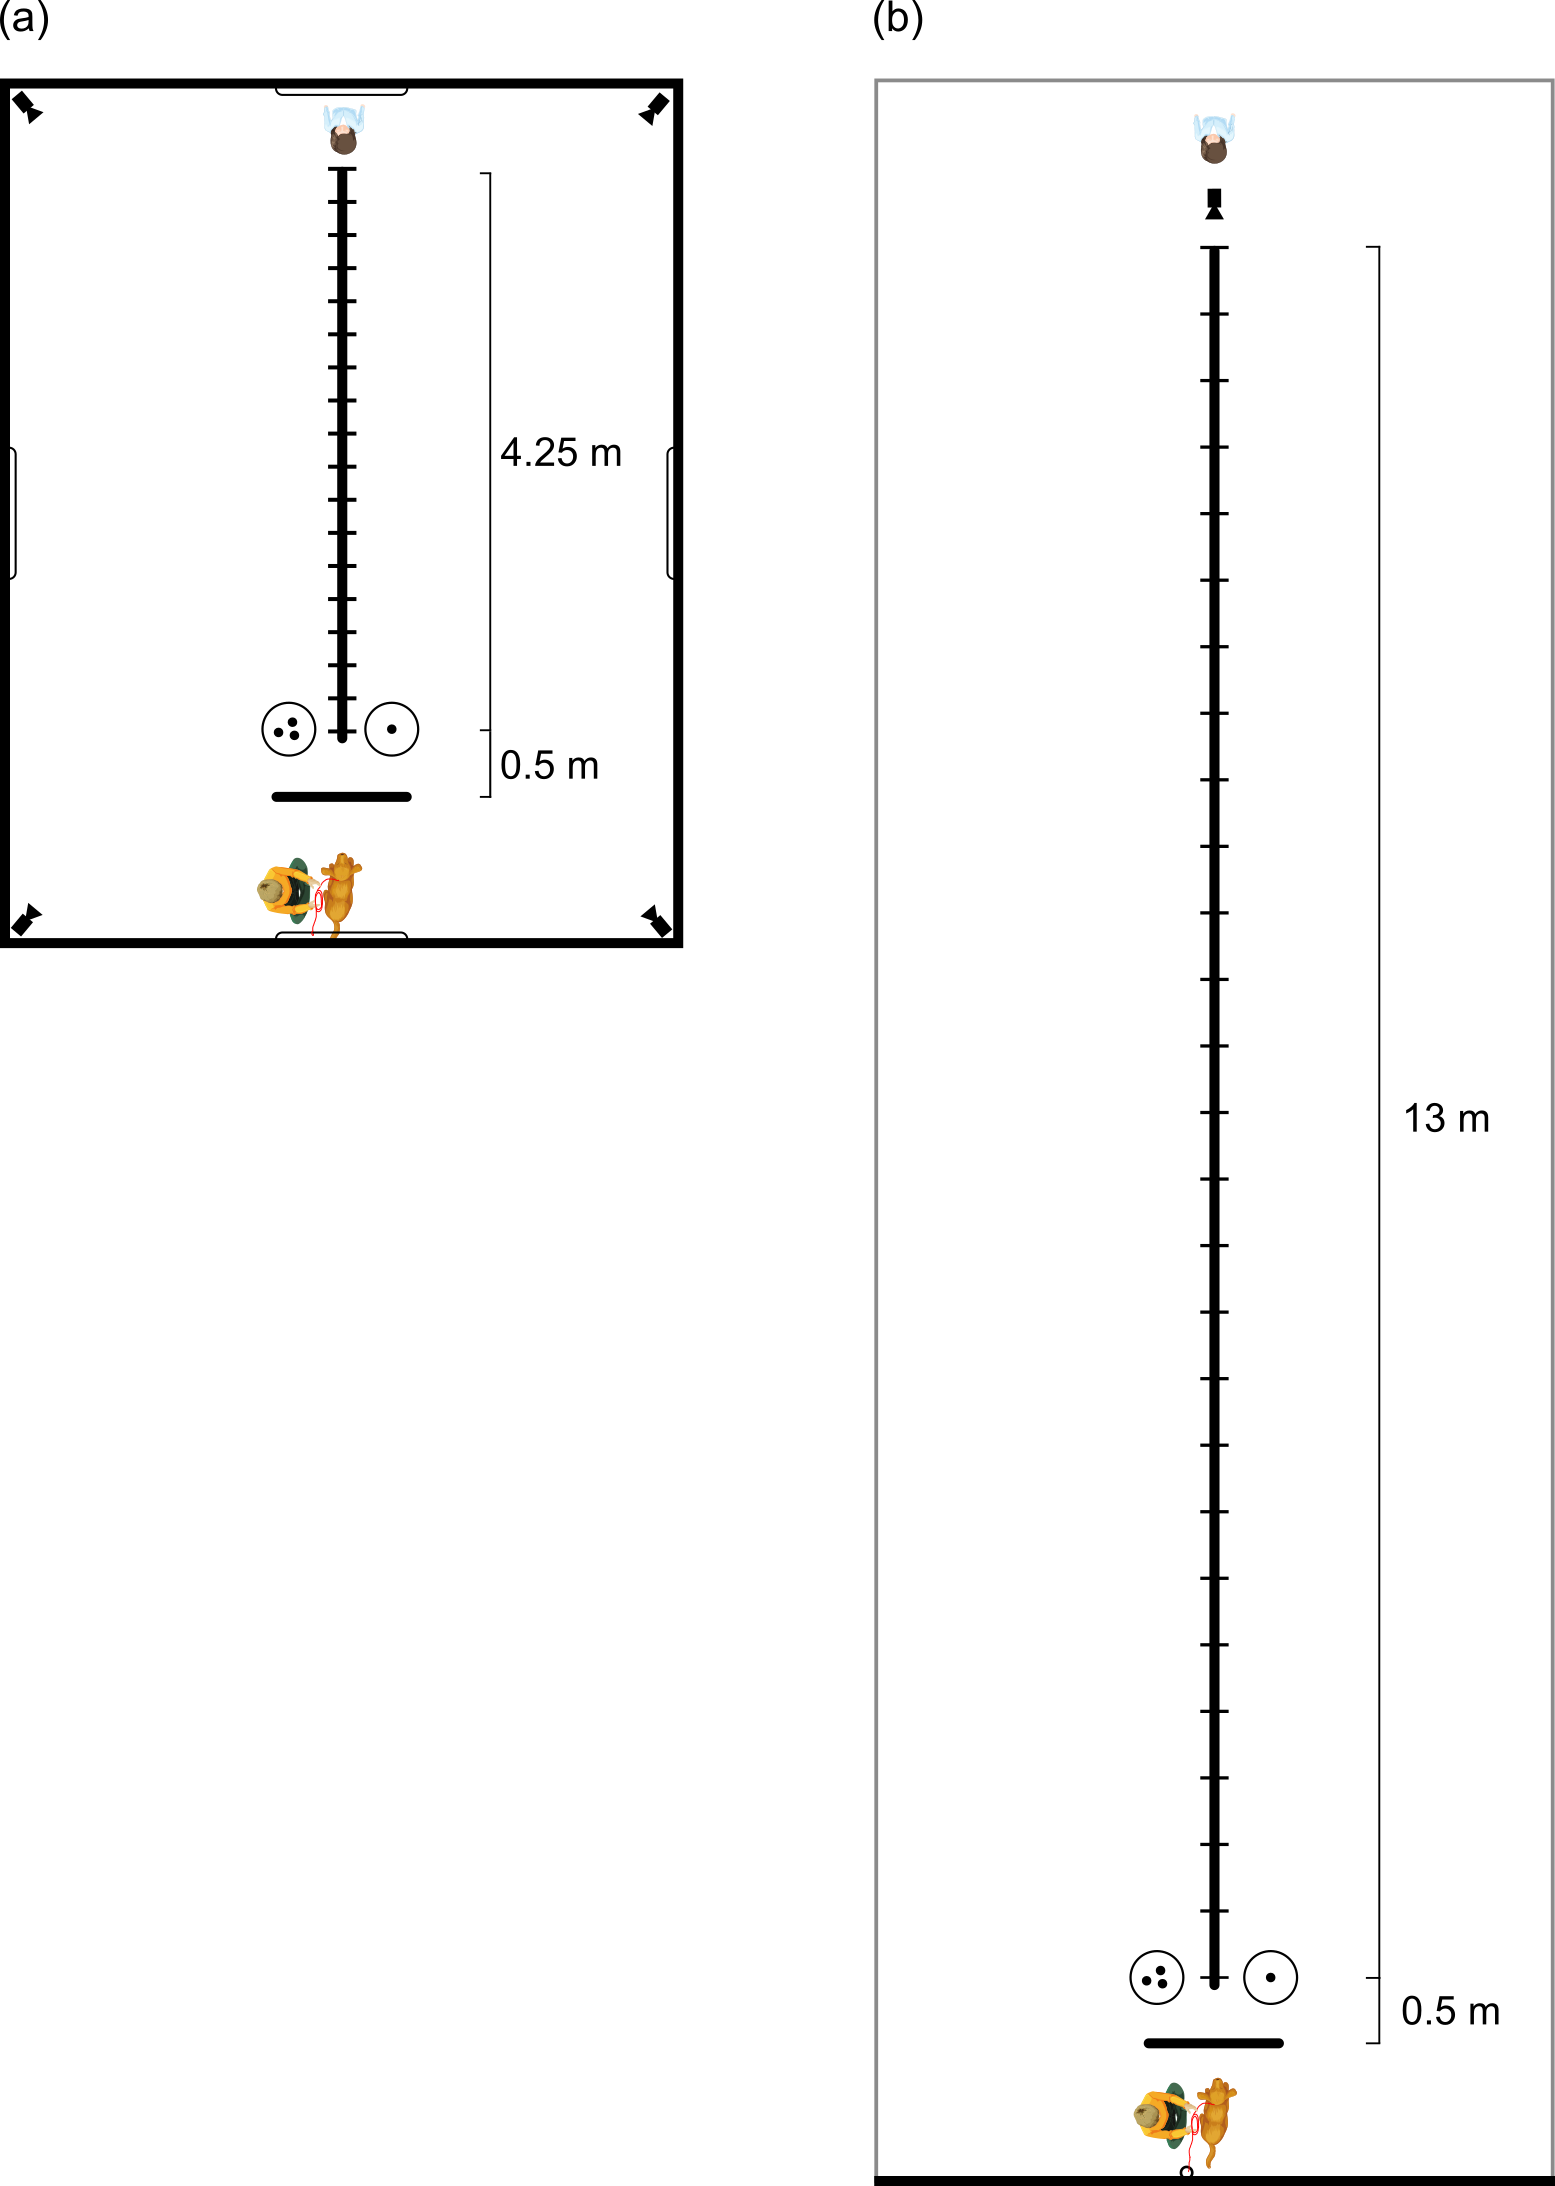
\includegraphics[width=0.8\linewidth]{figures/setup_study} 

}

\caption{Experimental set-up. (a) For Study 1, the illustration shows the entire room size.  (b) Study 2 was conducted in a much larger room, so only one wall (bottom) is illustrated. Dog figure from \href{https://vecteezy.com}{vecteezy.com} and experimenter figures adapted from art by \href{https://www.freepik.com/macrovector}{macrovector} on \href{https://www.freepik.com/free-vector/professions-top-view-colored-icons-set_3997920.htm}{freepik.com}.}\label{fig:exp-setup}
\end{figure*}

For Study 1, the behavioral tasks occurred in a 5.1 x 6.5 m room with video cameras mounted in all four corners. The experimental set-up included a starting area for the dog, a curtain to occlude the dog's view during trial set-up, an opaque barrier running perpendicular to the curtain, and plates for food rewards (Figure \ref{fig:exp-setup}a). We placed rewards on two equally sized circular plates of different colors (white or yellow) to enhance discrimination of the reward amounts. On each plate, we placed either the larger reward consisting of three small (1 cm\textsuperscript{3}) dog training treats or the smaller reward of one dog treat. The color of the plate containing each reward and the side of the small/large reward (right/left) were consistent within subjects across training and testing and were counterbalanced between subjects. Tape on the floor marked distances from the starting position in 0.25 m increments to a length of 4.25 m. Note that this distance is shorter than the maximum used by Brady et al. (2018) of 10 m. An opaque barrier running the length of the distances (4.25 m long, 50 cm high) ensured that once the dog selected an option, it could not see or obtain the unchosen option. An opaque curtain (80 cm high) separated the dog's starting area from the choice area and prevented them from observing the trial set-up. Two dogs could see over the curtain, which could have allowed the order of treat placement to affect their choices. The starting area included a metal bar attached to the wall with a 16 m leash attached to it.

For Study 2, the behavioral tasks occurred in a large gym where we used space approximately 10 x 16 m in size. The experimental set-up was very similar to that of Study 1 except (1) the distance ran up to 13 m (longer than Brady et al.'s (2018) length of 10 m), (2) the distances increased in steps of 0.5 m marked on a rope that ran the length of the 13 m center barrier, and (3) a single camera recorded the session from the end of the barrier (Figure \ref{fig:exp-setup}b). The starting area included a metal hook attached to the wall with the 16 m leash.

\hypertarget{surveys}{%
\subsection{Surveys}\label{surveys}}

For Study 1, while their dogs were completing the behavioral task, owners completed a Qualtrics survey on a tablet computer in a waiting room outside of the experimental testing room (owners could observe the behavioral testing via an external monitor). The survey consisted of questions about dog and owner demographics, information about dog-owner separation, the dog's general behaviors, training, feeding, and exercise habits, and six scales. For the purposes of this study, we included the following measures: dog age, dog sex, dog neuter status, dog weight, dog AKC Canine Good Citizen status, dog training ratings, dog obedience ratings, dog problem behaviors, dog impulsivity, dog separation anxiety, dog-owner relationship ratings, owner personality, owner cognitive ability, owner gender, and owner household income. We calculated Revelle's omega total (\(\omega_{T}\)) as our measure of internal consistency reliability of scales (Revelle \& Zinbarg, 2008; McNeish, 2018) unless these computations failed (e.g., for scales with only two items), in which case, we calculate Cronbach's \(\alpha\) (Table \ref{tab:reliability}).

\hypertarget{dog-training}{%
\subsubsection{Dog Training}\label{dog-training}}

To assess dog training, we asked owners to rate how well trained they thought their dogs were on a scale from 1 to 10 with 10 being the best.

\hypertarget{dog-obedience-and-behavioral-problems}{%
\subsubsection{Dog Obedience and Behavioral Problems}\label{dog-obedience-and-behavioral-problems}}

We used the Bennett and Rohlf (2007) scale, which assessed dog behavior problems with 24 questions on a seven-point scale with five subscales: disobedience, aggression, nervousness, destructiveness, and excitability.

We also used Hiby et al.'s (2004) scale to assess obedience and problem behaviors in dogs. Obedience was assessed on a five-point scale with seven specific tasks and an overall obedience score. Behavioral problems were assessed by participants indicating whether their dog had never, previously, or currently shown 13 behavioral problems.

\hypertarget{dog-impulsivity}{%
\subsubsection{Dog Impulsivity}\label{dog-impulsivity}}

The Dog Impulsivity Assessment Scale (Wright et al., 2011) assessed impulsivity in dogs using a five-point scale (plus ``don't know/not applicable''). The scale included 18 questions divided over three subscales (two questions are used in more than one subscale): behavioral regulation (Factor 1 in Wright et al.~2011), aggression (Factor 2), and responsiveness (Factor 3). We calculated the mean of the three subscales to generate a DIAS overall score (referred to as Overall Questionnaire Score or OQS in Wright et al.~2011).

\hypertarget{dog-owner-relationship}{%
\subsubsection{Dog-Owner Relationship}\label{dog-owner-relationship}}

The Monash Dog Owner Relationship Scale (Dwyer et al., 2006) used a seven-point scale to assess human-dog relationships by measuring how frequently owners engage in nine activities with their dogs.

\hypertarget{owner-personality}{%
\subsubsection{Owner Personality}\label{owner-personality}}

The brief Big-Five personality scale (Gosling et al., 2003) used a five-point scale to assess owner personality. The scale included 10 questions divided over five subscales: extraversion, agreeableness, conscientiousness, emotional stability, and openness to experience. While some of the internal consistency reliability values were low, (1) there were only two items per subscale (which forced us to calculate Cronbach's \(\alpha\) for reliability, as we could not compute Revelle's \(\omega_{T}\)), (2) our values are similar to the original study, and (3) the test-retest reliability and convergent correlations with a ten-item inventory were quite high in the original study.

\hypertarget{owner-cognitive-ability}{%
\subsubsection{Owner Cognitive Ability}\label{owner-cognitive-ability}}

The Cognitive Reflection Task (Frederick, 2005) used three multiple-choice questions to assess cognitive reflection in owners. The Berlin Numeracy Test (Cokely et al., 2012) used four multiple choice questions to assess owner numeracy. Scores for both tests were calculated by summing the number of correct responses. We summed the scores from these two tests to generate an index of cognitive ability that ranged from 0-7 (Stevens et al., 2021). If participants failed to answer any of the seven questions, their cognitive ability score was excluded from analyses that included this score (N = 26).

For Study 2, owners completed a Qualtrics survey at home prior to bringing their dogs in for testing. The survey consisted of the following measures: dog age, dog sex, dog neuter status, dog weight, dog AKC Canine Good Citizen status, dog training ratings, dog obedience ratings, dog impulsivity, dog separation anxiety, owner personality, owner gender, owner household income. We omitted the following measures from Study 1: dog problem behaviors, dog-owner relationship ratings, and owner cognitive ability.

Scales carried over from Study 1 included the Hiby et al. (2004) obedience score, the Dog Impulsivity Assessment Scale (Wright et al., 2011), and the brief Big-Five personality scale (Gosling et al., 2003). We replaced the training rating question with the C-BARQ trainability scale (Hsu \& Serpell, 2003), which is an eight-item questionnaire on a five-point scale. Reliability values for scales are provided in Table \ref{tab:reliability}.

\hypertarget{procedure}{%
\subsection{Procedure}\label{procedure}}

The experiment was conducted in a single approximately one-hour-long session. Dogs experienced a habituation phase, training phase, and testing phase. For Study 1, owners were with dogs during habituation but were outside the testing area during the training and testing phases. For Study 2, dogs were either dropped off for daycare or brought in for the study. If in daycare, the daycare staff brought the dogs over from the main building for testing and returned them after testing. For other dogs, the owner remained in their car while our staff retrieved the dog and brought them into the testing area. Therefore, owners were not present for testing in either study.

\hypertarget{habituation}{%
\subsubsection{Habituation}\label{habituation}}

To acclimate the dog to the space and equipment, one experimenter allowed the dog to walk around the waiting and testing areas for about 5 minutes. Dogs were allowed to sniff and walk around the curtain and barrier. Once dogs seemed accustomed to the space, two experimenters took the dog into the testing area. In Study 1, the owner left the testing area to take the survey in the waiting area, and the door between the two areas was closed. The experimenters then gave the dog treats to assess whether the dog was engaged with the experimenter or showed signs of stress from being separated from their owner. In Study 2, the habituation worked similarly to Study 1 but was slightly quicker because the owners were not present.

\hypertarget{training}{%
\subsubsection{Training}\label{training}}

The training phase occurred adjacent to the testing area to further acclimate the dog without the formal requirements of the testing situation (no curtain, no specific distances, etc.). In training, subjects chose between the smaller and larger reward amounts on plates. One experimenter (here labeled `presenter') placed the rewards on the plates and presented them about 0.5 m away from the subject. The other experimenter (here labeled `handler') sat next to the subject during the training, released the subject after presenting rewards, and encouraged them to choose a reward. Subjects were allowed to choose and consume one of the two options. The presenter immediately removed the unchosen option once the subject touched the chosen option. Training session bouts consisted of 12 trials for Study 1 (matching Brady et al.~(2018)) or 8 trials for Study 2 (shorter than Brady et al.~to speed training and reduce treat consumption before the main experiment). For the subject to move on to the testing phase, they had to select the larger treat amount in at least 10 out of the 12 trials (Study 1) or 5 of 8 trials (Study 2). For Study 1, they also had to select the larger reward in all of the last five trials of one training bout. As soon as subjects completed the requisite number of trials (10 or 5), the bout was stopped. Subjects could attempt up to five (Study 1) or three (Study 2) training bouts to reach the passing criteria. If the subject failed these training criteria in the required number of training bouts, the test was concluded and the dog did not advance to the testing phase.

\hypertarget{testing}{%
\subsubsection{Testing}\label{testing}}

Testing began following a short break after meeting training criterion. For this phase, the handler brought the subject over to the starting area, attached a long leash to the dog's collar, and directed the subject to face the curtain. Meanwhile, the presenter placed two plates 0.5 m from the starting position of the subject---one on either side of the central barrier. The same color of plates from the training phase were used here. The presenter then removed the curtain, walked to the opposite end of the barrier, and stood centered with the barrier with their back to the dog (Figure \ref{fig:exp-setup}). The presenter alternated which side of the barrier they walked down each round of testing to reduce side bias in results. After 4 seconds to view both options, the handler gave the command that the owner typically used to release from a stay position or said ``okay'' or ``go'' and released the slack on the leash. The dog had 30 seconds to choose a plate after being released. If the dog refused to look at the plates, refused to move, or moved in a different direction from the plates during this time, the trial was marked as no choice. If the dog looked at the plates during the 30 seconds, the handler repeated the release command once more and the dog was given 60 more seconds to make a choice. A choice was defined as the plate that the subject first touched or ate from. After the dog consumed the treats on the chosen plate, the handler called the subject back to the starting position or led them back with the leash. The handler kept the dog from getting the unchosen rewards by holding onto the leash and guiding the dog back to the starting position. The presenter then replaced the curtain and replenished the treats on the selected plate. A video of testing trials is available at the Open Science Framework (\url{https://osf.io/eb5m3/}).

Each time the dog selected the larger reward option, the plate was moved back one step (0.25 m for Study 1 and 0.5 for Study 2) in the subsequent trial. The testing phase concluded once the dog selected the smaller reward five times in a row or refused to select an option either three times in a row or five times total throughout the duration of testing. The response variable for this measure was the maximum distance traveled for the large reward.

\hypertarget{separation-anxiety}{%
\subsubsection{Separation anxiety}\label{separation-anxiety}}

If the subject appeared anxious with signs such as panting, drooling, whining, cowering, shaking, or walking to the door during any of the phases, training and testing were paused to re-acclimate the subject to the environment. In Study 1, the door to the waiting area was opened to allow access to the waiting room where the owner stayed for 10 minutes. Owners were prompted to not interact with subject during this period, and rewards were only given to the subject by experimenters in the testing room. After 10 minutes, the owners were asked to stand in the testing room while still ignoring the subject. Then the door to the testing room was closed. For 5 minutes, the experimenters continued to give rewards to the subject while allowing the subject to explore the room off leash. After 5 minutes, the subject was put on the leash used in testing for a minute at a time alternating between being on and off leash. The owner was then asked to leave the testing room. With the door closed, experimenters continued to give rewards to the subject for 15 minutes with 1 minute intervals of the subject being on the leash dispersed throughout the 15-minute period. Subjects were then allowed to go home without continuing to the training or testing phase. If the dog appeared to be more comfortable taking treats in the testing room and being separated from their owner at the end of the extended habituation, the subject was invited back to restart the study again from the beginning on a different day. If the dog did not show improvement in its comfort level, the subject was not invited back. For Study 1, four dogs were invited for a second attempt, but only one completed testing. For Study 2, two dogs were invited back, and one completed testing.

\hypertarget{data-analysis}{%
\subsection{Data analysis}\label{data-analysis}}

We used R (Version 4.2.0; R Core Team, 2022) and the R-packages \emph{BayesFactor} (Version 0.9.12.4.3; Morey \& Rouder, 2018), \emph{conflicted} (Version 1.1.0; Wickham, 2021), \emph{ggbeeswarm} (Version 0.6.0; Clarke \& Sherrill-Mix, 2017), \emph{ggdist} (Version 3.1.1; Kay, 2022), \emph{here} (Version 1.0.1; Müller, 2020), \emph{metaBMA} (Version 0.6.7; Heck et al., 2019), \emph{papaja} (Version 0.1.0.9999; Aust \& Barth, 2020), \emph{patchwork} (Version 1.1.1; Pedersen, 2020), \emph{psych} (Version 2.2.3; Revelle, 2020), and \emph{tidyverse} (Version 1.3.1; Wickham et al., 2019) for all our analyses. The manuscript was created using \emph{rmarkdown} (Version 2.14, Xie et al., 2018) and \emph{papaja} (Version 0.1.0.9999, Aust \& Barth, 2020). Data, analysis scripts, supplementary materials, and the reproducible research materials are available at the Open Science Framework (\url{https://osf.io/eb5m3/}).

We calculated Bayes factors (BF\textsubscript{10}) to provide the weight of evidence for the alternative hypothesis relative to the null hypothesis (Wagenmakers, 2007). For example, BF\textsubscript{10} = 3 means that the evidence for the alternative hypothesis is 3 times stronger than the evidence for the null hypothesis. BF\textsubscript{10} = 1/3 means that the evidence for the null hypothesis is 3 times stronger than the evidence for the alternative hypothesis. Bayes factors between \(1/3-3\) provide only anecdotal evidence, those between \(3-10\) or \(1/10-1/3\) provide moderate evidence, those between \(10-100\) or \(1/100-1/10\) provide strong evidence, and those above 100 or below 1/100 provide very strong evidence (Andraszewicz et al., 2015). Bayes factors were calculated with the \texttt{correlationBF()}, \texttt{ttestBF()}, and \texttt{anovaBF()} functions from the \emph{BayesFactor} package using default (noninformative) priors.

The sample size for both studies was determined by an optional stopping rule based on Bayes factors (Schönbrodt et al., 2017). We calculated the Bayes factors for the correlation between maximum distance traveled and the DIAS overall score and stopped analysis when it reached either 1/3 or 3. We analyzed the first 20 subjects and checked our Bayes factor every 2-5 subjects to determine whether one of the thresholds was met. This resulted in our final sample size of 65 subjects for Study 1 and 43 subjects for Study 2.

\hypertarget{results}{%
\section{Results}\label{results}}

\hypertarget{impulsivity}{%
\subsection{Impulsivity}\label{impulsivity}}

Dogs traveled a mean \(\pm\) SD distance of 1.69 m \(\pm\) 1.10 m (range: 0.25 \negthickspace \(-\) \negthickspace 4.25 m) in Study 1 and 1.81 m \(\pm\) 0.81 m (range: 0.50 \negthickspace \(-\) \negthickspace 4.50 m) in Study 2 (Figure \ref{fig:study-comp}a). The mean \(\pm\) SD Dog Impulsivity Assessment Scale (DIAS) overall scores were 0.48 \(\pm\) 0.09 (range: 0.31 \negthickspace \(-\) \negthickspace 0.70) in Study 1 and 0.47 \(\pm\) 0.06 (range: 0.36 \negthickspace \(-\) \negthickspace 0.63) in Study 2 (Figure \ref{fig:study-comp}b).

\begin{figure*}

{\centering 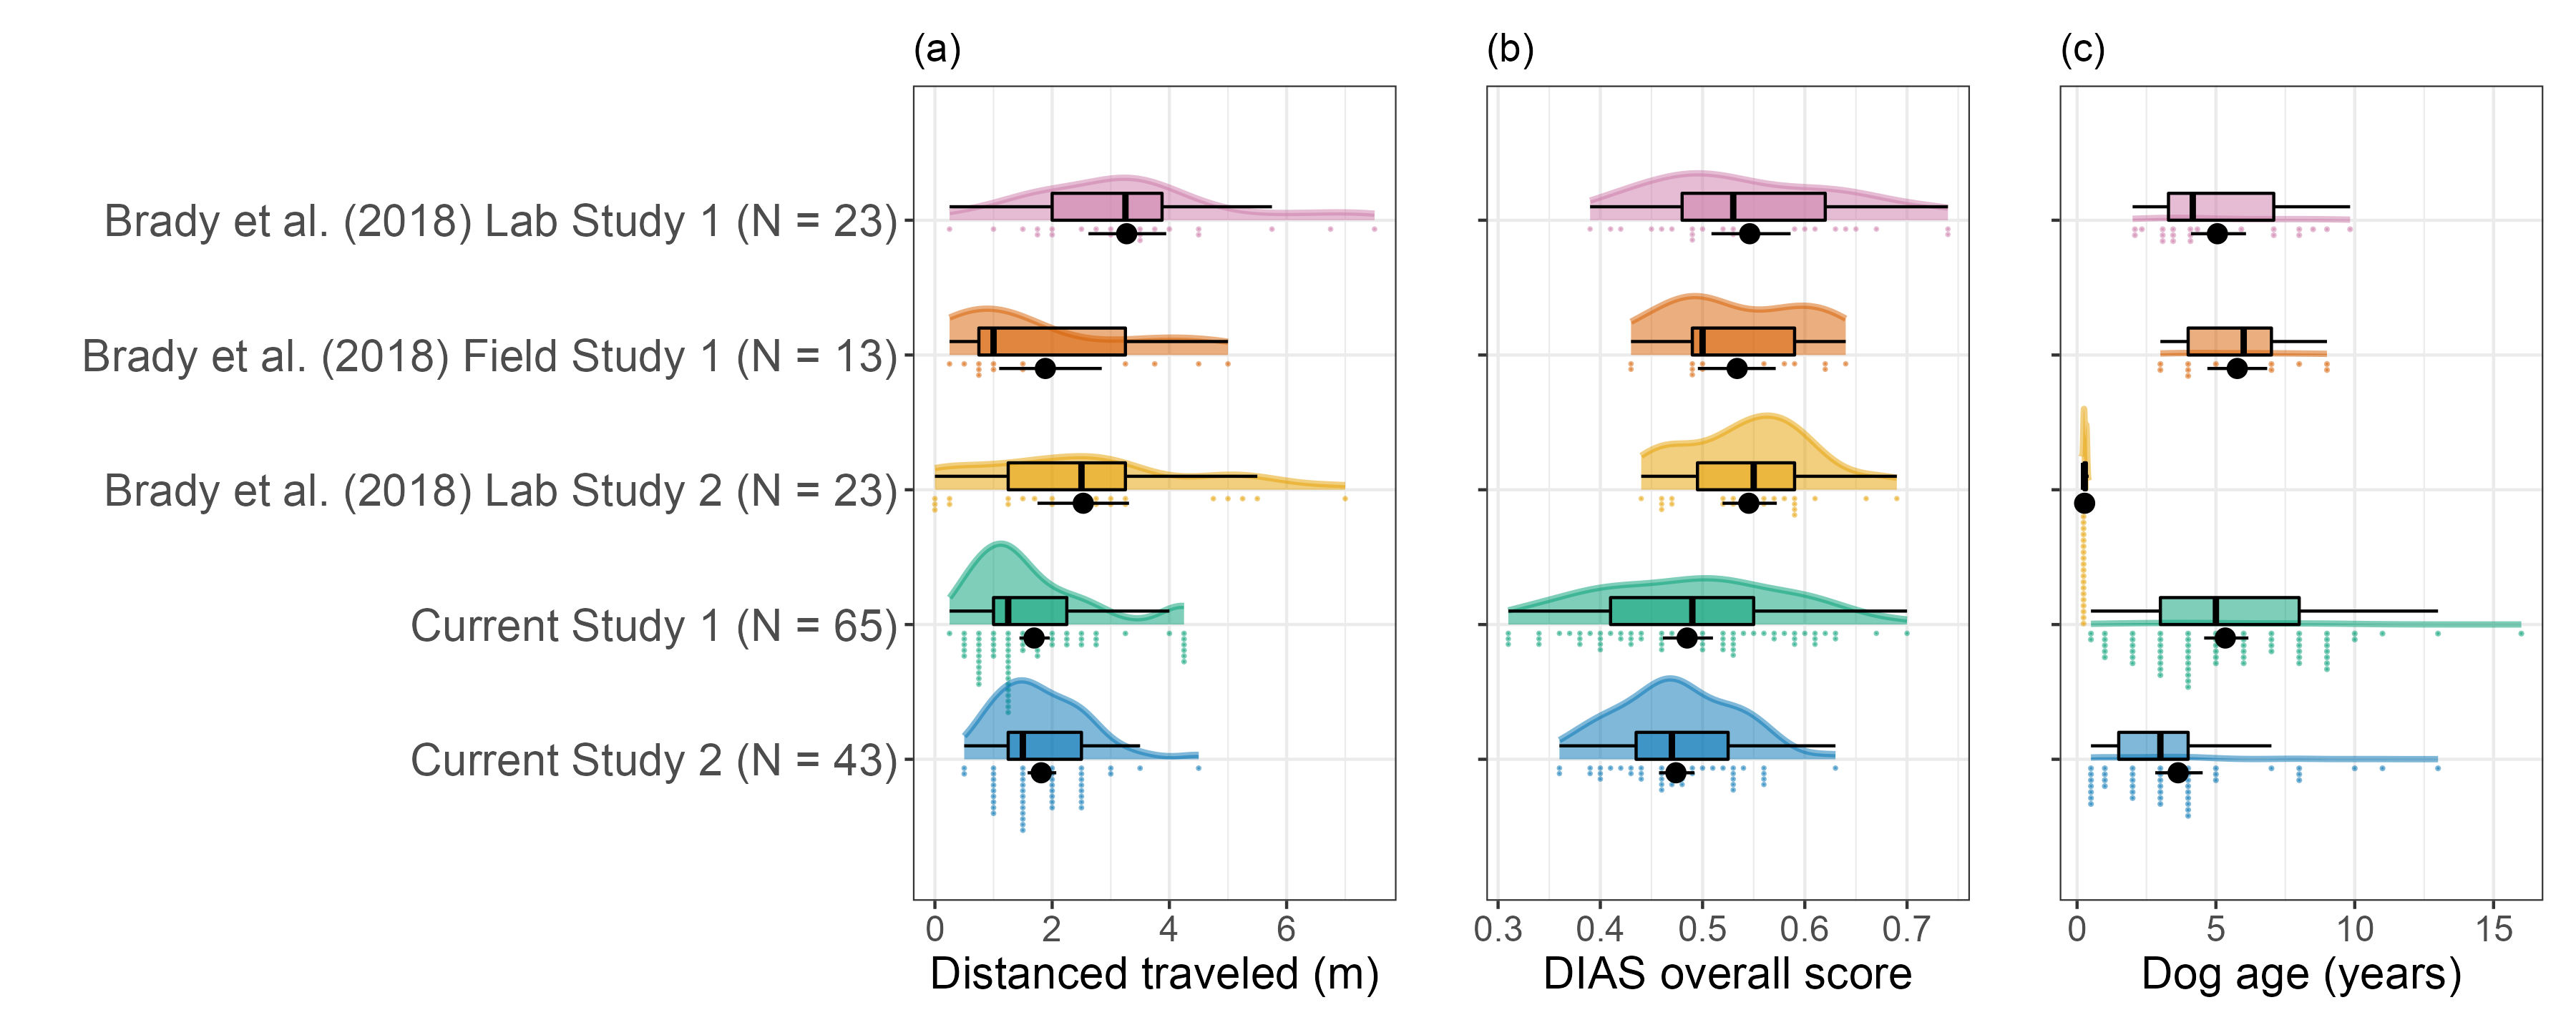
\includegraphics[width=1\linewidth]{figures/study_comparison} 

}

\caption{Distance traveled, DIAS overall score, and dog age across studies. Individual data points and summary statistics are shown for (a) distance traveled, (b) DIAS overall score, and (c) dog age for the Brady et al. (2018) and current studies. Colored dots represent individual dog data points, filled shapes represent density distributions, black dots and error bars represent mean and 95\% confidence intervals, boxes represent interquartile range, lines within boxes represent medians, and whiskers represent 1.5 times the interquartile range.}\label{fig:study-comp}
\end{figure*}

Our primary analysis correlated the maximum distance traveled by the dog with the owner's DIAS overall score. Neither study showed evidence for a correlation between distance traveled and owner assessments of impulsivity (Study 1: \(r = -0.10\), 95\% CI \([-0.34, 0.15]\), \(t(63) = -0.80\), \(p = 0.429\), \(\mathrm{BF}_{\textrm{10}} = 0.38\); Study 2: \(r = 0.04\), 95\% CI \([-0.26, 0.34]\), \(t(41) = 0.26\), \(p = 0.798\), \(\mathrm{BF}_{\textrm{10}} = 0.35\); Figure \ref{fig:dias}).

\begin{figure*}

{\centering 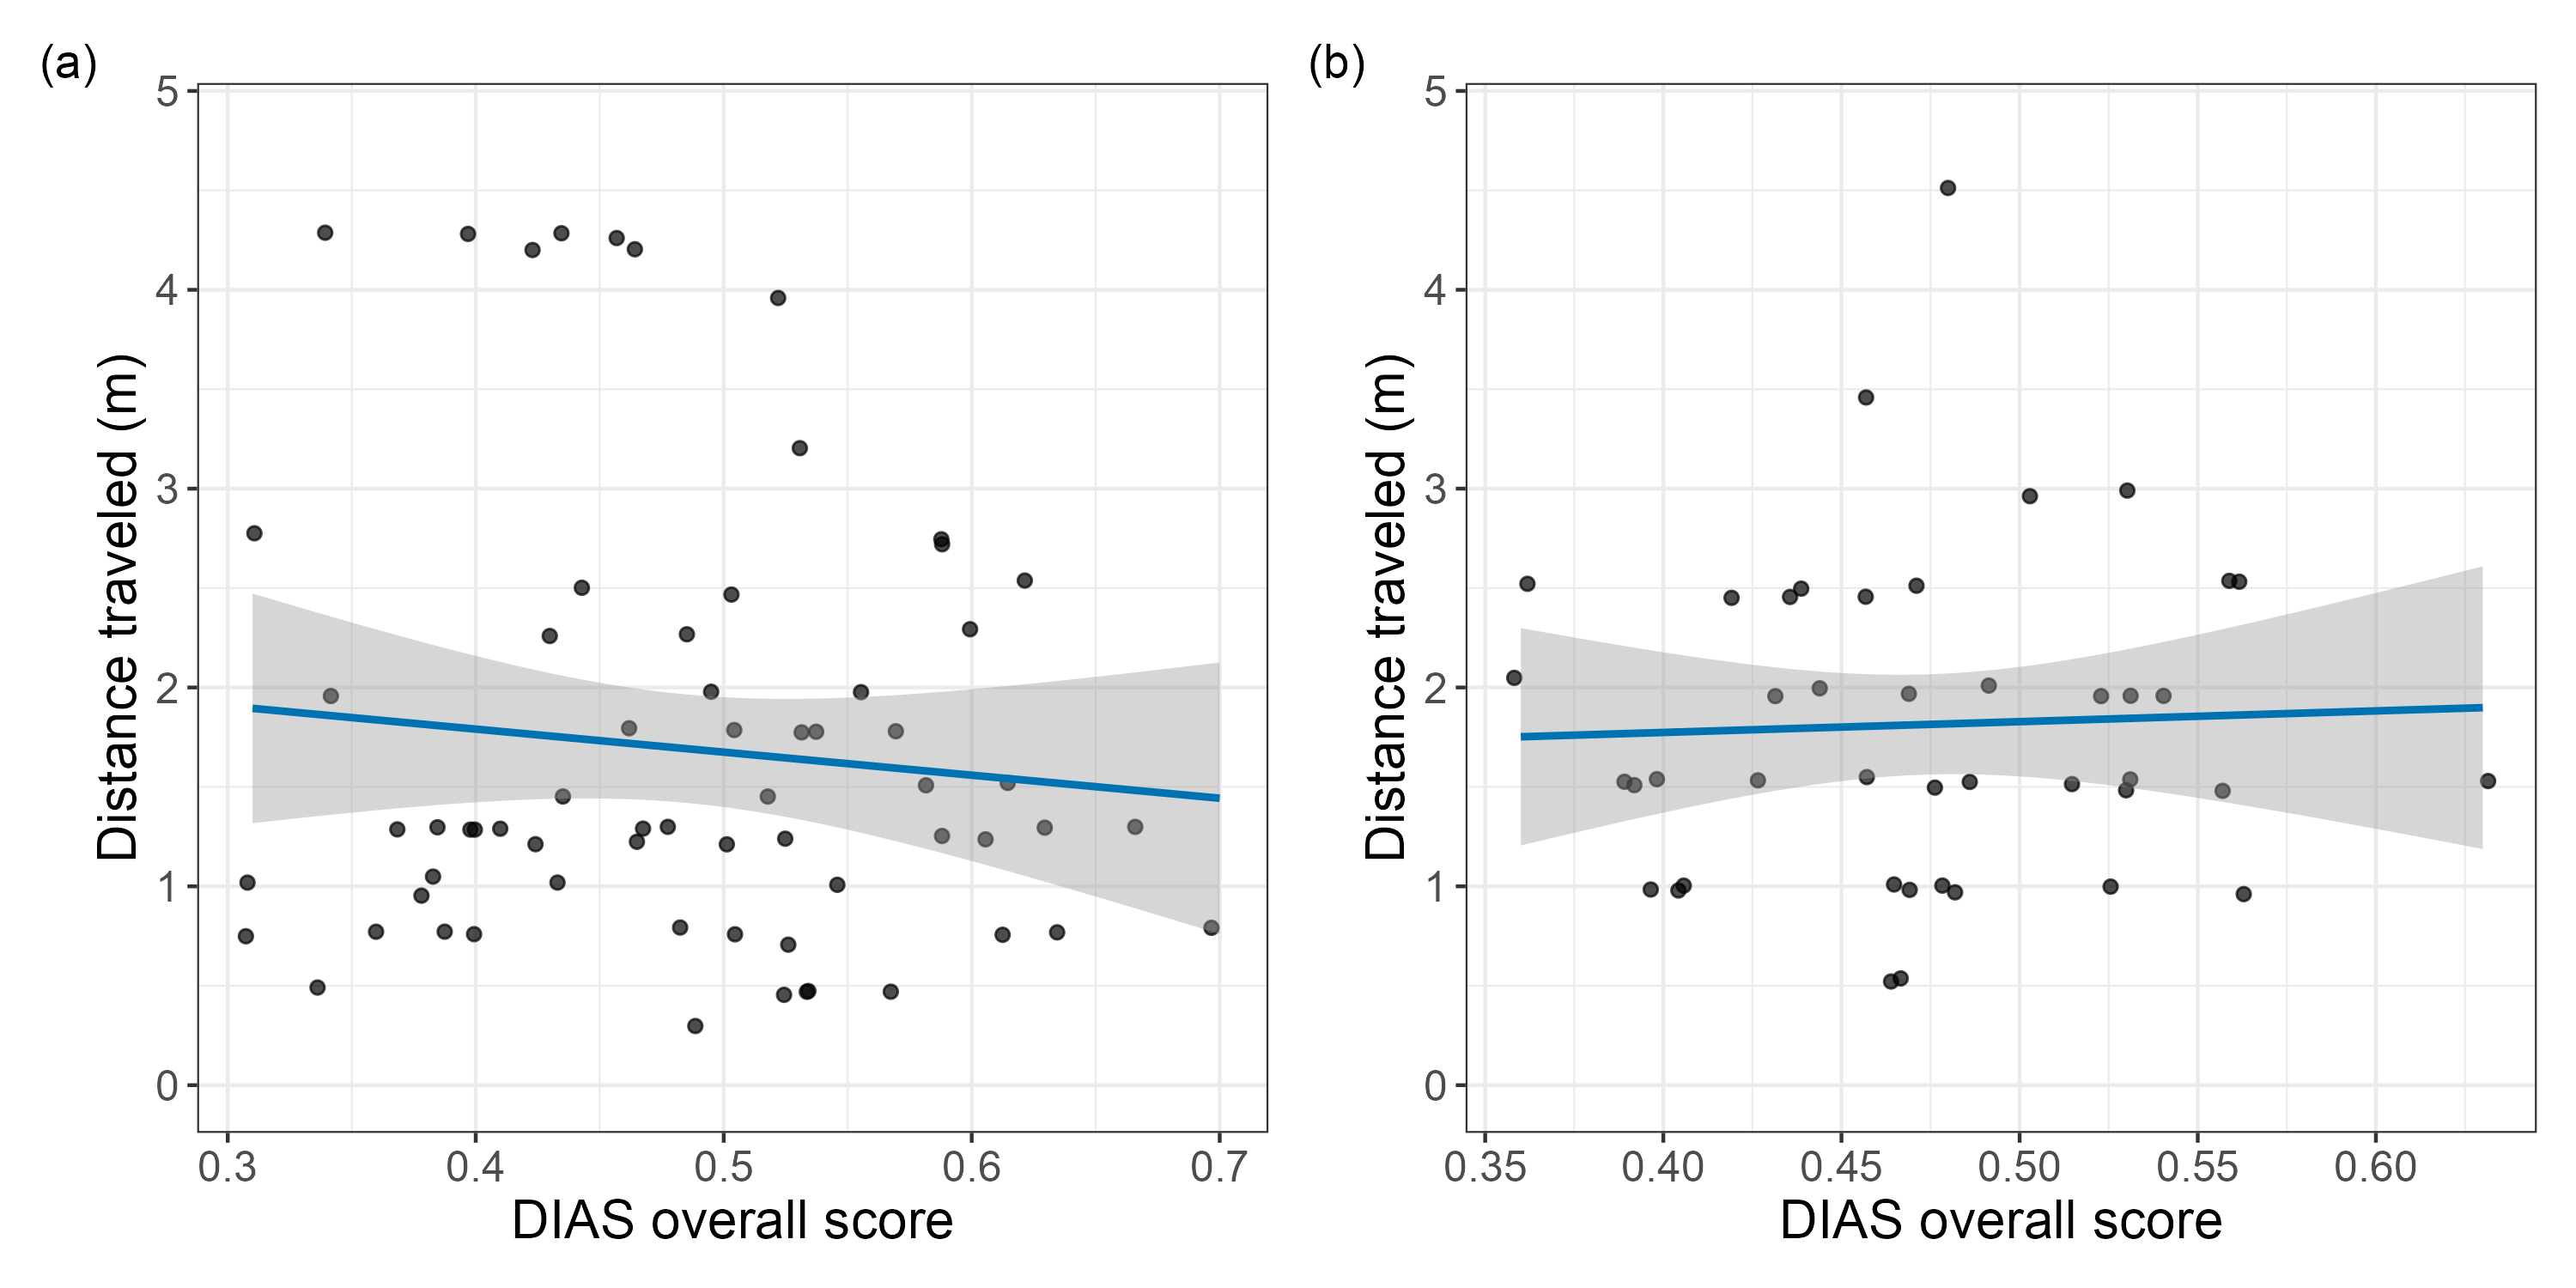
\includegraphics[width=1\linewidth]{figures/distance_dias_overall} 

}

\caption{Relationship between distance traveled and DIAS overall score. Scatterplots of distance traveled and DIAS overall score for (a) Study 1 and (b) Study 2 showed no evidence for a correlation. Dots represent individual dog data points, lines represent best fitting linear regression models, and bands represent 95\% confidence intervals around the regression models.}\label{fig:dias}
\end{figure*}

For both studies, we collected data until the Bayes factor for this correlation reached either 1/3 or 3. Unfortunately, due to a coding error in the analysis script in which we did not remove sessions for training experimenters, we stopped both studies slightly before reaching either threshold (Study 1: N = 65, \(\mathrm{BF}_{\textrm{10}} = 0.38\); Study 2: N = 43, \(\mathrm{BF}_{\textrm{10}} = 0.35\)). Because optional stopping is not a problem for Bayes factor analyses (Rouder, 2014), we can combine the data sets from the two studies to calculate Bayes factors for exploratory analyses of the overall effect. Despite the longer room and maximum distance in Study 2, the studies did not differ in either the distribution of distances traveled by the dogs (\(\Delta M = -0.12\), 95\% CI \([-0.49, 0.24]\), \(t(104.68) = -0.66\), \(p = 0.509\), \(\mathrm{BF}_{\textrm{10}} = 0.25\), Figure \ref{fig:study-comp}a) or the distribution of DIAS overall scores (\(\Delta M = 0.01\), 95\% CI \([-0.02, 0.04]\), \(t(105.85) = 0.74\), \(p = 0.462\), \(\mathrm{BF}_{\textrm{10}} = 0.25\), Figure \ref{fig:study-comp}b). However, dogs in the second study were younger on average than those in the first study (\(\Delta M = 1.70\), 95\% CI \([0.50, 2.90]\), \(t(95.00) = 2.80\), \(p = 0.006\), \(\mathrm{BF}_{\textrm{10}} = 5.77\), Figure \ref{fig:study-comp}c). With the combined data, there is moderate evidence for the null hypothesis of no correlation between dog travel distance and owner reports of impulsivity (\emph{r} = \(-0.07\), \(\mathrm{BF}_{\textrm{10}} = 0.28\)).

Analyses of the DIAS subscales in both studies also showed (anecdotal) evidence for no correlations with distance traveled (0.34 \(\leq\) BF\textsubscript{10} \(\leq\) 0.46; Figure \ref{fig:dias-all}). Combining the studies showed moderate evidence for no correlation between distance traveled and behavioral regulation (\emph{r} = \(-0.05\), \(\mathrm{BF}_{\textrm{10}} = 0.25\)), aggression (\emph{r} = \(0.07\), \(\mathrm{BF}_{\textrm{10}} = 0.28\)), or responsiveness (\emph{r} = \(-0.07\), \(\mathrm{BF}_{\textrm{10}} = 0.28\)).

\hypertarget{other-measures}{%
\subsection{Other measures}\label{other-measures}}

For exploratory analyses of other factors that may relate to distance traveled, we combined data from the two studies and only present Bayes factors for analyses. In terms of dog demographic characteristics, distance traveled did not relate to dog sex, weight, age, or AKC Canine Good Citizen status (Figure \ref{fig:dog-char}). For dog behavior measures, distance traveled did not relate to Bennett and Rohlf (2007) problem behavior scores, Hiby et al. (2004) obedience score, training score, or the owner report of separation anxiety (Figure \ref{fig:dog-behavior}). For owner characteristics, distance traveled did not relate to owner extraversion, agreeableness, stability, openness, cognitive ability, or whether they had other dogs in the household (Figure \ref{fig:owner-char}). We had insufficient evidence to robustly assess potential relationships with the Monash dog owner relationship scores and owner conscientiousness.

\hypertarget{study-comparison}{%
\subsection{Study comparison}\label{study-comparison}}

Because our findings did not replicate those of Brady et al. (2018), we conducted an exploratory comparison of their and our studies. Since our two studies do not differ in distance traveled or DIAS overall score (see Impulsivity section), we combined the data across studies for each of these measures. Our combined data have shorter distances traveled than Brady et al.'s Lab Study 1 (\(\Delta M = -1.53\), 95\% CI \([-2.30, -0.76]\), \(\mathrm{BF}_{\textrm{10}} > 1000\)) and their Lab Study 2 with puppies (\(\Delta M = -0.79\), 95\% CI \([-1.65, 0.07]\), \(\mathrm{BF}_{\textrm{10}} = 7.49\)) but comparable travel distances to their Field Study (\(\Delta M = -0.14\), 95\% CI \([-1.15, 0.86]\), \(\mathrm{BF}_{\textrm{10}} = 0.32\); Figure \ref{fig:study-comp}a). Our DIAS overall score values were lower than those of their Lab Study 1 (\(\Delta M = -0.07\), 95\% CI \([-0.11, -0.02]\), \(\mathrm{BF}_{\textrm{10}} = 26.96\)) and their Lab Study 2 (\(\Delta M = -0.06\), 95\% CI \([-0.10, -0.03]\), \(\mathrm{BF}_{\textrm{10}} = 47.65\)), with anecdotal evidence for a difference with their Field Study (\(\Delta M = -0.05\), 95\% CI \([-0.10, -0.01]\), \(\mathrm{BF}_{\textrm{10}} = 2.19\); Figure \ref{fig:study-comp}b).

To further compare studies, we conducted an exploratory meta-analysis of Brady et al.'s (2018) three studies, Mongillo et al.'s (2019) study, and our two studies. For Brady et al.'s studies and our studies, we used the provided correlation coefficients and sample sizes. For Mongillo et al., we used the correlation between DIAS scores and overall proportion choice for larger, more distant option. We converted these correlation coefficients to Fisher's \(z\) scale and calculated standard errors based on the equation \(SE = 1 / \sqrt{(N - 3)}\) (Borenstein et al., 2009). We then input these values into the \texttt{meta\_bma()} function in the \emph{metaBMA} package (Heck et al., 2019) with default priors for Fisher's \(z\) values (Cauchy distribution with \texttt{scale=0.354} for the effect size and inverse gamma with \texttt{shape=1} and \texttt{scale=0.075} for \(\tau\)). This function allows us to test not only if there is evidence of an effect but also evidence for between-study heterogeneity (Gronau et al., 2021), that is, whether there is variation in true effect sizes across studies. We then converted the Fisher's \(z\) values back to correlation coefficients for presentation. This analysis used model averaging to calculate (1) a Bayesian estimate of the effect size across all studies, (2) a Bayes factor for evidence supporting the hypothesis of an effect, and (3) a Bayes factor for evidence supporting the presence of between-study heterogeneity (Gronau et al., 2021). This analysis found a model-averaged effect of \(r = -0.11\) (95\% credibility interval {[}-0.27, 0.04{]}), which provided anecdotal evidence of no correlation between distance traveled and DIAS score across all studies (\(\mathrm{BF}_{\textrm{10}} = 0.51\); Figure \ref{fig:forestplot}). It also found anecdotal evidence of no between-group heterogeneity (\(\mathrm{BF}_{\textrm{10}} = 0.74\)).

\begin{figure*}

{\centering 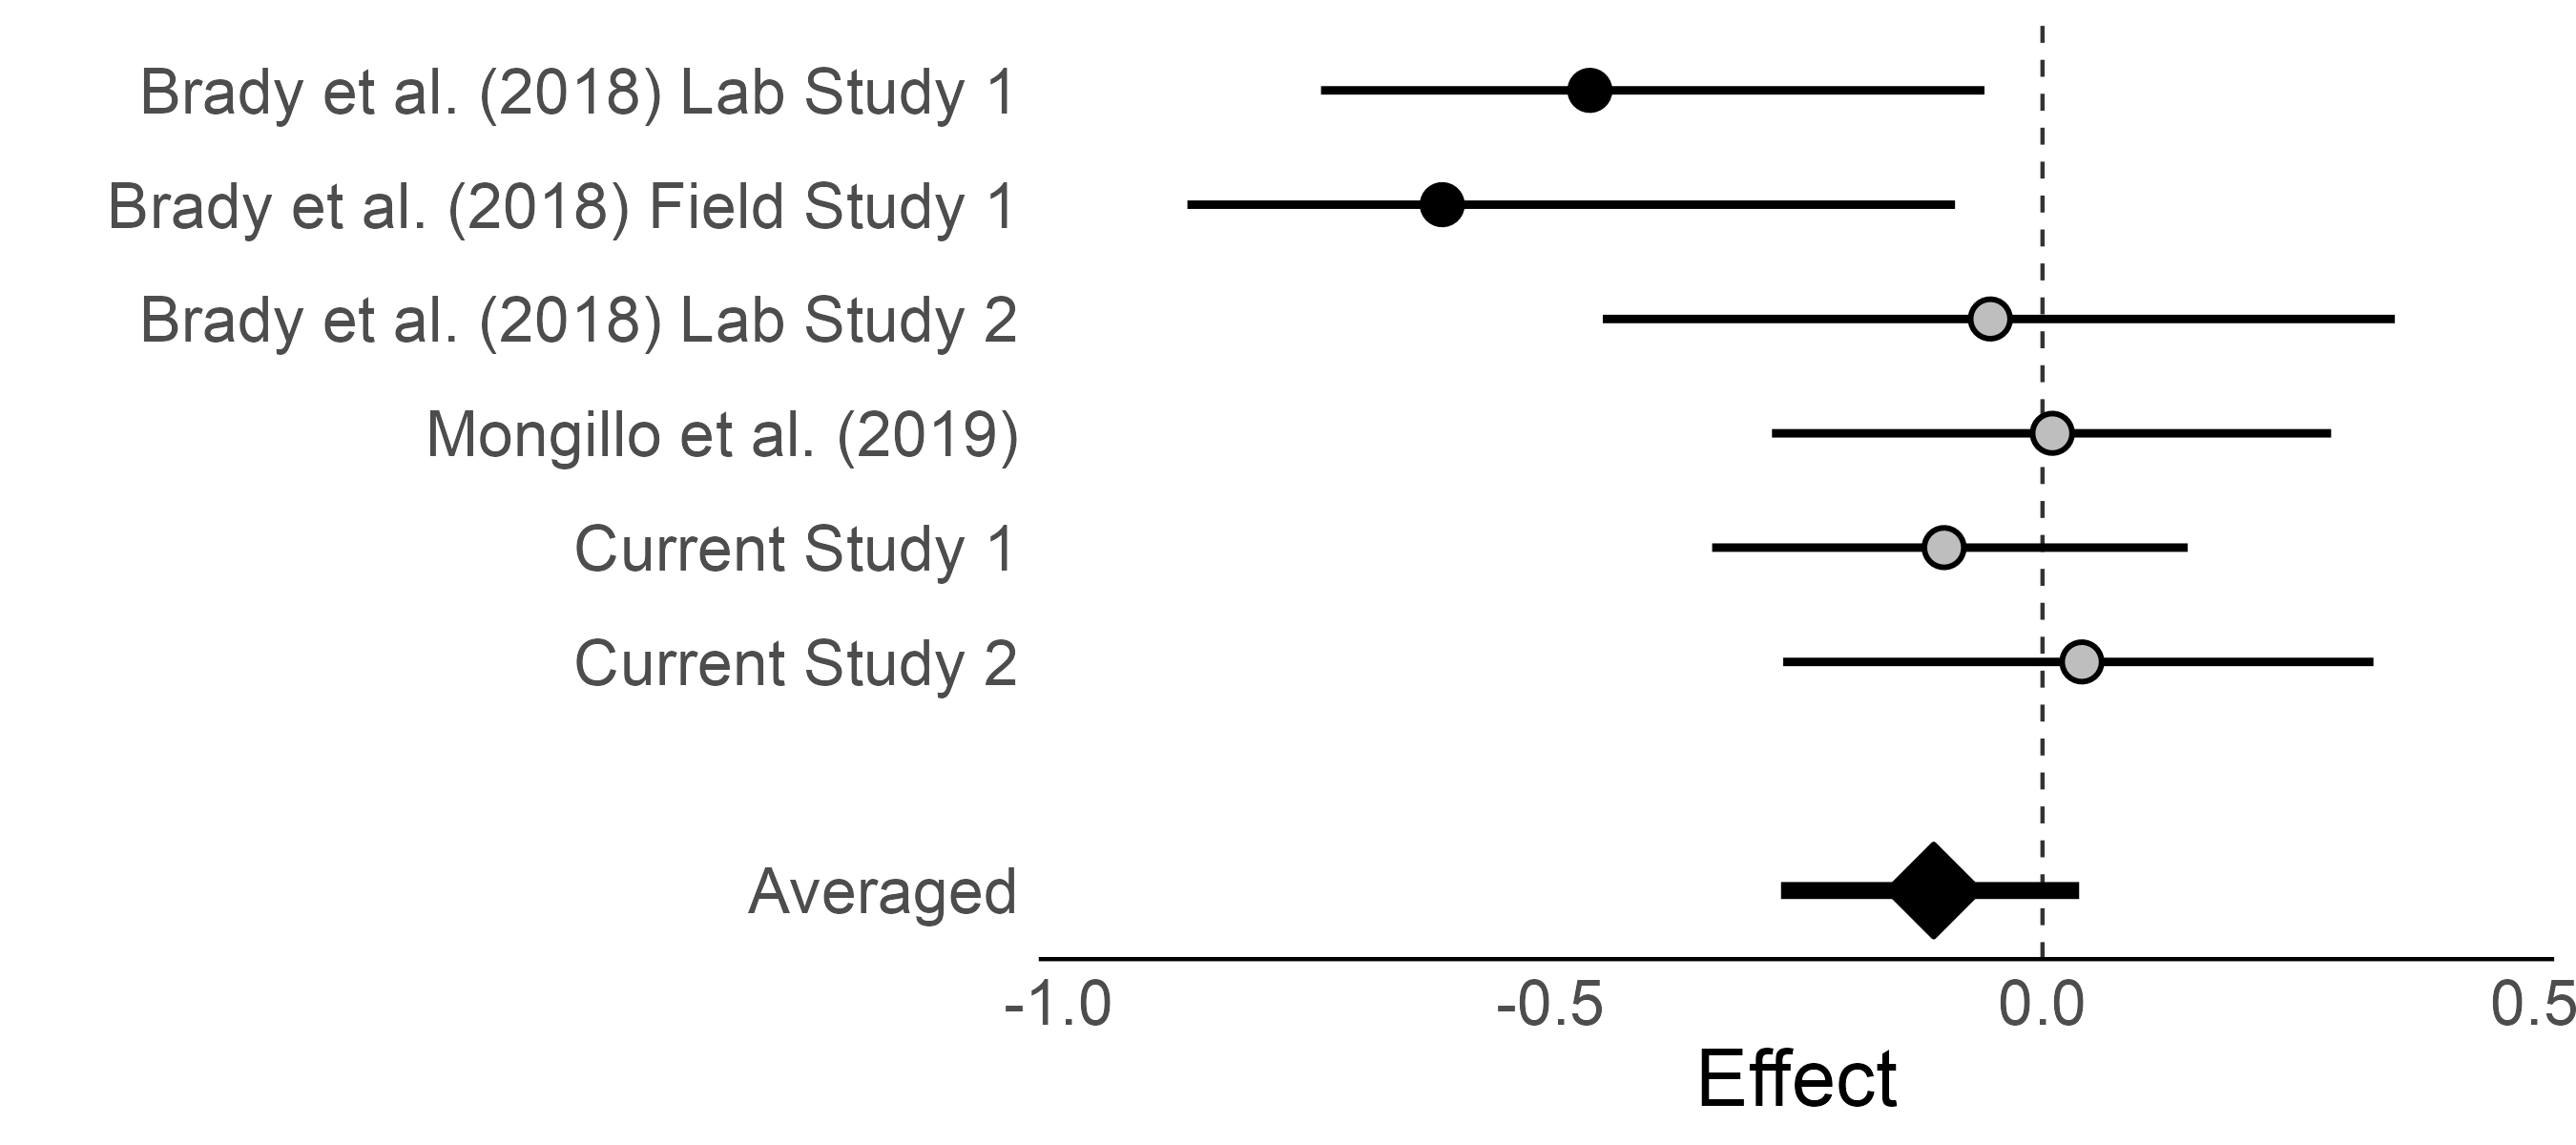
\includegraphics[width=1\linewidth]{figures/forestplot_bf} 

}

\caption{Forest plot of meta-analysis. Plot shows effect sizes (correlation coefficients, $r$) and 95\% confidence/credibility intervals around effect sizes for Brady et al. (2018), Mongillo et al. (2019), and current studies. Black dots represent effect sizes different from 0, grey dots represent effect sizes not different from 0, and the black diamond represents the Bayesian model-averaged effect size over all studies. Study error bars represent confidence intervals, and model-averaged error bars represent credibility interval.}\label{fig:forestplot}
\end{figure*}

\hypertarget{discussion}{%
\section{Discussion}\label{discussion}}

In two studies, we found no relationship between the distance traveled by dogs in a spatial impulsivity task and the owner reports of dog impulsivity. In fact, the distance traveled did not relate to any measures of dog behavior, dog characteristics, or owner characteristics.

\hypertarget{replication-differences}{%
\subsection{Replication differences}\label{replication-differences}}

Our two studies differed in four major ways. First, the training criteria differed, with subjects needing to choose the larger option in 10 of 12 trials in Study 1 and 5 of 8 trials in Study 2. For Study 2, choosing larger on 5 of 8 trials does not pass a binomial test (using \(\alpha\) = 0.05), so it is possible that subjects did not discriminate the amounts as well in Study 2. To examine whether the criteria difference influenced performance, we assessed whether subjects completed training faster in Study 2. Subjects required a mean±standard deviation of 1.58 \(\pm\) 1.09 training bouts to advance in Study 1 and 1.31 \(\pm\) 0.58 bouts in Study 2. Thus, there was anecdotal evidence for no difference in number of training bouts required across the two studies (\(t(91.58) = 1.58\), \(p = .117\), \(\mathrm{BF}_{\textrm{10}} = 0.51\)). This difference in training criteria likely did not influence the testing results since the distance traveled did not differ between studies. As a second difference, Study 2 used a longer maximum distance (13 m) and steps (0.5 m) in a larger room than Study 1 (maximum: 4.25 m, steps: 0.25 m). Study 1 used a distance more similar to Mongillo et al.'s (2019) maximum distance of 3.5 m, whereas Study 2 was more similar to Brady et al.'s (2018) maximum distance of 10 m. Despite this large difference in maximum distances and room size, the distance traveled did not differ between studies. A third difference between studies was that Study 1 drew participants exclusively from our database, whereas the second study included database participants and dog owners who used the dog daycare where we conducted the experiment. Thus, the daycare dogs were more familiar with the personnel and testing area than the other dogs. Nevertheless, we found anecdotal evidence that daycare and database dogs did not differ in the distance traveled or DIAS scores (BFs \textless{} 1), though the sample size for daycare dogs was small (N = 15). And, again, the distance traveled by dogs did not differ between studies. Finally, dogs in Study 2 were on average younger than those in Study 1. Yet, age did not influence distance traveled. Thus, though there were a few key differences between our studies, we reliably replicated the same lack of an effect across both studies.

We failed to replicate Brady et al.'s (2018) finding that owner reports of impulsivity matched their dogs' distance traveled in a spatial impulsivity task. Our results align with Mongillo et al.'s (2019) demonstration of no relationship, though we use different methods to assess spatial impulsivity. Interpreting the inability to replicate results is difficult (Stanley \& Spence, 2014; Maxwell et al., 2015), so we evaluate our replication based on LeBel et al.'s (2019) recommendations for replications. Our \emph{methodological similarity} is high, as we directly aimed to replicate the methods of Brady et al. (2018). We used the same operationalizations of dependent and independent variables (DIAS overall score and maximum distance traveled), in contrast to Mongillo et al. (2019) who used different methods for eliciting choice and used proportion choice for the most distant option as the dependent variable. In terms of \emph{replication differences}, we addressed a possible difference of a shorter distance in Study 1 by employing a longer distance in Study 2. Nevertheless, the distances traveled by dogs did not differ between our studies, though they were slightly shorter distances than Brady et al.~found. Our DIAS overall scores appeared to be the same as Brady et al.~There is no \emph{investigator independence} issue, as all investigators from this study are completely independent from the original study. We aim for \emph{study transparency} by posting all data on Open Science Framework (\url{https://osf.io/eb5m3/}); however, the study was not pre-registered. We facilitate \emph{analytic result reproducibility} by posting our analysis scripts with our data, allowing others to reproduce our analyses. We allow evaluations of \emph{auxiliary hypotheses} by including reliability of our measures (Table \ref{tab:reliability}), which all exceeded reliability measures reported in the original instrument development (Wright et al., 2011). Given that we have met these six criteria, our results qualify as ``No signal - inconsistent'' in LeBel et al.'s terminology. That is, our replication effect size 95\% confidence intervals include 0 (Study 1: \(r = -0.10\), 95\% CI \([-0.34, 0.15]\); Study 2: \(r = 0.04\), 95\% CI \([-0.26, 0.34]\)) but not the original effect size point estimates from Brady et al.'s adult studies (\emph{r} = \(-0.46\) and \(-0.61\)).

To compare results across all of the studies published thus far, we conducted an exploratory meta-analysis that combined our data with those of Brady et al. (2018) and Mongillo et al. (2019). This meta-analysis found that, across these six studies, the overall effect size is in the direction demonstrated by Brady et al.~However, the calculated effect size is substantially smaller than the original studies and the credibility interval includes 0. The Bayesian analysis found anecdotal evidence for no between-study heterogeneity and no correlation between distance traveled and DIAS scores. But because the evidence is only anecdotal, we cannot draw strong conclusions based on these results. Moreover, we must acknowledge the assumptions and limitations of Bayesian meta-analyses. First, we used a single set of priors for the Bayesian model based on the defaults suggested for Fisher's \(z\) scale by Heck et al. (2019). Other priors might result in different outcomes. Second, the sample size for this meta-analysis was relatively small with only six studies. More studies are needed to have better estimates of the effect sizes. Moreover, selection of studies is critical. For instance, we included Brady et al.'s Lab Study 2---which focused on puppies---to maximize the number of studies included in the analysis. But an argument could be made to exclude this study since it focused on puppies (for our purposes, removing this study does not change any of our findings). Finally, a key weakness of meta-analyses is that they are distorted by publication bias. Given the relatively recent publication date of Brady et al. (2018), it is unlikely that there are many additional studies at the moment that have been conducted but not published. Nevertheless, failures to replicate are not published at the same rate as confirming replications (Francis, 2012; Makel et al., 2012; Martin \& Clarke, 2017), and the resulting publication bias may generate a larger overall effect size than is accurate (Simonsohn et al., 2014; Friese \& Frankenbach, 2020). In summary, the meta-analysis does not resolve the presence of an effect, so more studies are needed.

Why might we see such variability across studies? The first possibility is that we did not accurately replicate Brady et al. (2018). However, we made every effort to replicate the methods described in their article. Though our first study used a smaller space and maximum distance, we rectified this in the second study. Otherwise, our methods were very similar to the original study.

A second possibility is that we sampled a different subset of the dog population than the original study. One clear way that this could happen could be based on age. Brady et al.'s two adult studies (that showed the effect) involved dogs that were \(2-10\) years old (mean \(\pm\) SD = \(5.3 \pm 2.3\)), whereas dogs in our studies ranged from \(0.5-16\) (mean \(\pm\) SD = \(4.7 \pm 3.2\)) years old. However, trimming our data down to \(2-10\) year old dogs (\(N = 42\), mean \(\pm\) SD = \(5.0 \pm 2.4\)) did not change the results for the correlation between maximum distance traveled and DIAS overall score for the combined study data (\(r = -0.05\), \(\mathrm{BF}_{\textrm{10}} = 0.27\)), indicating that dog age differences across the samples do not account for effect differences.

Relatedly, there could be breed differences between study samples. From the tables in Brady et al. (2018), it appears as though the vast majority of dogs in their samples are purebred (5 of 37 or 13.5\% are listed as `crossbreed'). In our samples, 37 out of 108 (34.2\%) were listed as mixed breed (data set includes owners' descriptions of breed). This is likely a low estimate, as we did not explicitly ask if the dogs were purebred. Breed composition matters because breeds may differ in their impulsivity (Fadel et al., 2016; Gerencsér et al., 2018), though this is not always the case (Lit et al., 2010). Moreover, owners may have expectations about breed differences in impulsivity. Therefore, differences in breed composition in samples may result in different relationships between owner reports and dog impulsivity.

A third possibility is that we sampled a different subset of the owner population than Brady et al. (2018). While demographic information about dogs is commonly provided in the dog behavior literature, information on the owners is often not. This is important because as researchers, we are selectively sampling from a subset of dog owners---those who have the time, funds, and interest to bring their dogs in for testing. These samples are not representative and may have critical influences on generalizability, so we need to encourage more thorough reporting of owner information to capture potential differences between studies. We provide summary information on the owners' gender identity, marital status, and household income category in Table \ref{tab:demographics} and individual values in our data set. In hindsight, we would like to have collected information about age, employment status, and time spent at home with their dogs. Factors such as age, marital status, income, employment status, and time spent with the dog are important variables to consider when examining owner knowledge about their dogs and impulsivity specifically. If our lab sampled a different subset of owners than Brady et al., our sample may have different knowledge about their dogs' impulsivity, which could drive the study differences. Alternatively, a different subsample of owners may select or train their dogs differently, which can result in more variability in impulsivity levels, again resulting in study differences. Given the critical importance of owners in raising and training the dogs in our samples, canine science researchers should improve and standardize the collection and availability of information about owners.

The dog and owner sample differences imply that our lab may simply draw a different subset of dogs and owners from a common population compared to the other studies. However, a fourth possibility is that there are real differences between the populations to draw from; that is, cultural differences may exist between our populations and those of Brady et al. (2018). Cultures differ in their attitudes toward and beliefs about dogs (Bradshaw \& Goodwin, 1999; Serpell, 2004) and their experiences and interactions with dogs (Wan et al., 2009; Amici et al., 2019). Our study was completed in the United States (US), whereas Brady et al.~was conducted in the United Kingdom (UK), two countries that differ in the frequency of dog ownership. In 2021, approximately 53\% of US households had dogs (American Pet Products Association, 2021), compared to 33\% of UK households (Pet Food Manufacturers' Association, 2021). The two countries also differ in many aspects of dog welfare, health care, attitudes, policies, and laws (Houpt et al., 2007). Though there are few direct comparisons of US and UK dog owners, there is some evidence that veterinarians' beliefs about breed characteristics are shared for some breeds but differ for other breeds between the two countries (Bradshaw \& Goodwin, 1999). Differences in attitudes and beliefs about dogs could influence how owners train, relate to, and interact with their dogs. These differences in turn could influence both how impulsive their dogs are, as well as how well owners know their dogs' behavioral traits. For instance, US owners are more likely than UK owners to spay or neuter their dogs (Diesel et al., 2010; Trevejo et al., 2011). Because neutered male dogs may be more impulsive than non-neutered males (Fadel et al., 2016), different frequencies of neutered males may influence distributions of impulsivity scores. In our sample, 94.7\% of the males were neutered. Though Brady et al.~do not report their neuter rate, it was likely much lower than ours. However, UK and Italian owners share similar attitudes toward dogs (Lakestani et al., 2011), but Mongillo et al. (2019) did not replicate the effects of Brady et al.~either. Thus, potential cultural differences between study populations should be further investigated.

\hypertarget{implications}{%
\subsection{Implications}\label{implications}}

Along with Mongillo et al. (2019), our results call into question the robustness of the relationship between performance on a spatial impulsivity task and an owner's report of dog impulsivity more generally. Four out of six studies on this topic do not show a relationship (Figure \ref{fig:forestplot}). A meta-analysis does not yield definitive evidence in either direction, though it provides anecdotal evidence favoring no relationship. What does this mean for canine impulsivity?

Brady et al. (2018) investigated the relationship between spatial impulsivity and DIAS because they were interested in developing a measure of impulsivity that could be assessed quickly; that is, it did not require the repeated interactions needed to offer an accurate assessment of impulsivity via the DIAS. This could be useful especially in settings such as animal shelters, where quickly assessing dog impulsivity can trigger additional training or help find a match with potential adopters. Our study comparison suggests that the spatial impulsivity task may not provide a broadly reliable measure of impulsivity for these purposes. We discussed the possibility of cultural/country differences potentially explaining the divergent findings across studies. This implies that the spatial impulsivity task may be a useful general measure of impulsivity in some situations (e.g., UK households) but not others. To estimate how generalizable it is as a measure of impulsivity, the task should be replicated more both within and outside of the UK.

Not finding a relationship between spatial impulsivity and DIAS scores, however, is perhaps not surprising given other information about impulsivity. Impulsivity is a multi-faceted concept that refers to many different cognitive and motivational processes (Evenden, 1999; Reynolds et al., 2006; Stevens, 2017b). In humans, while there are some correlations across different measures of impulsivity, there are also many aspects of impulsivity that are unrelated (Whiteside \& Lynam, 2001; Weber et al., 2002; DeYoung, 2011). Someone who is impulsive in the sense that they may gorge themselves on a decadent dessert may not be impulsive in the sense of engaging in unprotected sex. Similarly, the literature in dogs has failed to find relationships among different behavioral measures of impulsivity and inhibitory control, despite numerous studies searching for a consistent behavioral trait of impulsivity (Bray et al., 2014; Fagnani et al., 2016; Brucks, Marshall-Pescini, et al., 2017; van Horik et al., 2018). Thus, the fact that we found no noticeable relationship between spatial impulsivity and owner reports of impulsivity matches a broader set of results on this phenomenon across species.

The spatial impulsivity task likely taps into what would be considered \emph{impulsive choice} rather than \emph{impulsive action}, which refers to the inability to inhibit a response (Stevens, 2017b). Many of the classic inhibition tasks would fall under the impulsive action category (Bray et al., 2014; Brucks, Marshall-Pescini, et al., 2017; van Horik et al., 2018). Impulsive choice refers to situations in which individuals must choose between different reward amounts with different associated costs (e.g., intertemporal choice or risky choice, Stevens, 2017b). For spatial impulsivity, the cost is the time and energy required to obtain the larger rewards (Stevens et al., 2005). Having well-defined descriptions of concepts related to impulsivity may help clarify how concepts are related as well as help refine what types of methods best capture the concepts.

Given the distinction between impulsive choice and action, it is important to understand what aspects of impulsivity the DIAS captures. For instance, studies on impulsive action have not demonstrated relationships with DIAS (Mitcham, 2015; Brucks, Marshall-Pescini, et al., 2017; Cavalli et al., 2018). Research using measures of impulsive choice such as intertemporal choice (Wright et al., 2012; Riemer et al., 2014) and spatial impulsivity (Brady et al., 2018) have shown a relationship with DIAS; however, others have failed to show relationships in these types of impulsive choice tasks (Fagnani et al., 2016; Brucks, Soliani, et al., 2017; Mongillo et al., 2019). The items included in the behavioral regulation component of DIAS ask owners generally about whether their dogs are impulsive, are patient, are persistent, think before they act, demonstrate repetitive behaviors, have control over how they respond, and calm down quickly after getting excited. Interestingly, these items tend to be either rather general or vague terms (impulsive, patient) or refer to impulsive action (think before they act, have control over responses). Thus, one might not expect strong relationships with measures of impulsive choice, especially spatial impulsivity, which has minimal connection to the items in the DIAS. Without a stronger connection between DIAS and behavioral measures of impulsivity, it is difficult to use the DIAS or the impulsivity tasks in an applied setting, for instance, to make recommendations about using either measure as information for finding an appropriate home for a dog.

\hypertarget{challenges-and-opportunities}{%
\subsection{Challenges and opportunities}\label{challenges-and-opportunities}}

Both direct and conceptual replications can be difficult to implement. We applaud Brady et al. (2018) for facilitating replication by offering detailed descriptions of their methods and providing the individual data for their findings. Clear, thorough descriptions of methods are critical to providing the opportunity for others to replicate methods. We would also encourage the public posting of example videos of trials to further clarify methods. Additionally, individual-level data provided by Brady et al.~facilitated our ability to compare the studies more directly in ways that cannot be compared with simple summary statistics. Publicly available trial-level data can be even more beneficial to others, as it offers more granular levels of analysis and more flexible statistical models such as generalized linear models.

We advocate for leveraging aspects of open science to further advance research on dog behavior and cognition (Stevens, 2017a; Beran, 2018). One of the first ways to improve the robustness of our findings is to recruit larger sample sizes. For correlational work in particular, small sample sizes can result in spurious relationships (Schönbrodt \& Perugini, 2013; Loken \& Gelman, 2017). While many experts are hesitant to offer more statistical rules of thumb, larger samples are better, and this is especially relevant in dogs given their variation in size and breed-specific selection differences. Carefully considering in advance what your sample size will be (Lakens, 2022) or using sequential hypothesis testing with Bayes factors as we do here (Schönbrodt et al., 2017) is critical to collecting large enough samples to yield robust results. In addition, formally pre-registering or at least informally pre-specifying analysis plans is critical for reducing researcher degrees of freedom in analyzing data (Wagenmakers et al., 2012). For instance, including in the analysis the dog that Brady et al. (2018) excluded due to a diagnosis of hip dysplasia after the study dramatically changes the outcome of their analysis, dropping the correlation coefficient from \(r = -0.46\) to \(r = -0.37\) and increasing the p-value from 0.028 to 0.077. At small sample sizes, Pearson correlations are vulnerable to outliers and robust analyses are required (Wilcox, 2004). Flexibility in outlier exclusions combined with small sample sizes can reduce robustness of results, substantially influencing interpretations of our studies.

Producing a robust, reliable canine science requires implementing transparent and open research practices (Stevens, 2017a; Beran, 2018). One initiative that provides this opportunity in canine science is the ManyDogs Project (\url{http://manydogs.org/}). This project is a consortium of dog researchers around the globe interested conducting the same studies in all of their sites (ManyDogs et al., 2021). This not only provides much larger sample sizes than are reasonable at individual sites but also allows for direct comparison of similarities/differences across breeds and countries. Moreover, the project is devoted to open science practices including pre-registration of hypothesis, methods, and analysis plans, as well as public posting of data. Even if a researcher does not directly participate in it, the ManyDogs Project provides a model for transparent and open practices for canine science.

Finally, we raise an open secret in the dog cognition world. These studies were our lab's first research projects that involved bringing dogs into the lab for behavioral testing. One unexpected finding from this endeavor was how many dogs did not advance to the actual experiment. Out of 220 dogs that we recruited in total, 96 advanced to testing. A 56.4\% failure-to-advance rate was unexpectedly high. While some of the dogs failed to advance because they were not treat motivated or failed to reliably prefer the larger reward in training, the vast majority of these dogs seemed to not engage in the task because they were too focused on their owner being out of the room. In Study 1, we intentionally kept owners in a different room to avoid cuing or interactions with the dog. However, many dogs seemed to exhibit separation anxiety with their owners out of the room. After noticing the high drop-out rate, we began asking owners if their dogs experienced separation anxiety. But informally, this did not seem to predict whether their dog would advance or not. We attempted to minimize this issue in Study 2 by starting with dogs who were already at the dog daycare and therefore should not experience separation anxiety. However, we only recruited a moderate number of dogs this way and recruited the remaining subjects through our database again.

We raise the issue of separation anxiety here to (1) be explicit about this happening and (2) highlight that the data are coming from an even smaller slice of the dog population than it may seem. Not only are we primarily recruiting a subset of people who are interested in and willing to come in to do the testing, but we are collecting data from a subset of those whose dogs are comfortable being in a different room from their owners. Thus, our findings are not necessarily representative of dogs generally, and this could potentially be another population difference between our sample and that of Brady et al. (2018). Furthermore, the recent COVID-19 pandemic has resulted in people staying home more, which could potentially influence separation anxiety in dogs (Heirs \& Graham, 2021; Harvey et al., 2022). Further work is needed to investigate this, but it is important in considering recruitment and interpretation of dog cognition research. Going forward, we recommend allowing owners in the testing room with their dogs to reduce the drop-out rate. This requires additional thought and planning about ways to avoid owners intentionally and unintentionally cuing their dogs. However, the potential benefits of higher success in data collection will likely outweigh the costs of additional time and thought required to minimize cuing effects.

\hypertarget{conclusion}{%
\subsection{Conclusion}\label{conclusion}}

Impulsivity is a critical feature of canine science. Finding easy measures of impulsivity could benefit dog training, obedience, welfare, breeding, and re-homing. However, impulsivity is a multi-faceted construct, and being impulsive in one context may not predict impulsivity in another context. We found that impulsivity in a spatial context did not relate to the owner's overall assessment of a dog's impulsivity. While this did not replicate the findings of Brady et al. (2018), it did match Mongillo et al.'s (2019) finding of no relationship. There are many potential reasons for our inability to replicate Brady et al., ranging from potential methodological and population differences to larger cultural differences between sites. This outcome highlights the importance of implementing robust open science practices across canine science to help translate our results into practice in ways that benefit both owners and dogs.

\hypertarget{acknowledgments}{%
\section{Acknowledgments}\label{acknowledgments}}

This research was funded in part by the National Science Foundation (NSF-1658837) and by private funds donated to the University of Nebraska Foundation. We would like to thank Dian Quist from Kenl Inn for allowing us to use her facilities and recruit from the dogs in her dog daycare. We also thank the Kenl Inn staff for helping bring the dogs to the testing area.
We are grateful to the following assistants for helping to test the dogs:
Jessica Barela,
Meredith Batten,
Toria Biancalana,
Katie Carey,
Hunter DeBoer,
Rose Felice,
Haley Hays,
Billy Lim,
Brianna Moser,
McKenna Rezny,
Joelle Sanger,
Taylor Schendt, and
Destiny Vail.

\hypertarget{author-contributions}{%
\section{Author Contributions}\label{author-contributions}}

\textbf{Stevens:} Conceptualization, Data Curation, Formal Analysis, Funding Acquisition, Methodology, Project Administration, Resources, Supervision, Visualization, Writing -- Original Draft Preparation. \textbf{Mathias:} Investigation, Project Administration, Supervision, Writing -- Review \& Editing. \textbf{Herridge:} Investigation, Project Administration, Supervision, Writing -- Review \& Editing. \textbf{Hughes-Duvall:} Investigation, Project Administration, Supervision, Writing -- Review \& Editing. \textbf{Wolff:} Investigation, Supervision, Writing -- review \& editing. \textbf{Yohe:} Investigation, Writing -- Review \& Editing.

\textbf{Conflict of interest:} The authors declared that no conflicts of interest exist.

\textbf{Data Availability:} The data and analysis code are available at: \url{https://doi.org/10.17605/osf.io/eb5m3}.

\hypertarget{references}{%
\section{References}\label{references}}

\scriptsize

\begingroup

\hypertarget{refs}{}
\begin{CSLReferences}{1}{0}
\leavevmode\vadjust pre{\hypertarget{ref-AmericanPetProductsAssociation.2021}{}}%
American Pet Products Association. (2021). \emph{2021-2022 {APPA National Pet Owners Survey}}. https://americanpetproducts.org/pubs\_survey.asp.

\leavevmode\vadjust pre{\hypertarget{ref-Amici.etal.2019}{}}%
Amici, F., Waterman, J., Kellermann, C. M., Karimullah, K., \& Bräuer, J. (2019). The ability to recognize dog emotions depends on the cultural milieu in which we grow up. \emph{Scientific Reports}, \emph{9}(1), 1--9. \url{https://doi.org/10.1038/s41598-019-52938-4}

\leavevmode\vadjust pre{\hypertarget{ref-Andraszewicz.etal.2015}{}}%
Andraszewicz, S., Scheibehenne, B., Rieskamp, J., Grasman, R., Verhagen, J., \& Wagenmakers, E.-J. (2015). An introduction to {Bayesian} hypothesis testing for management research. \emph{Journal of Management}, \emph{41}(2), 521--543. \url{https://doi.org/10.1177/0149206314560412}

\leavevmode\vadjust pre{\hypertarget{ref-R-papaja}{}}%
Aust, F., \& Barth, M. (2020). \emph{{papaja}: {Prepare} reproducible {APA} journal articles with {R Markdown}}. \url{https://github.com/crsh/papaja}

\leavevmode\vadjust pre{\hypertarget{ref-Bennett.Rohlf.2007}{}}%
Bennett, P. C., \& Rohlf, V. I. (2007). Owner-companion dog interactions: {Relationships} between demographic variables, potentially problematic behaviours, training engagement and shared activities. \emph{Applied Animal Behaviour Science}, \emph{102}(1), 65--84. \url{https://doi.org/10.1016/j.applanim.2006.03.009}

\leavevmode\vadjust pre{\hypertarget{ref-Beran.2018}{}}%
Beran, M. (2018). Replication and pre-registration in comparative psychology. \emph{International Journal of Comparative Psychology}, \emph{31}(0).

\leavevmode\vadjust pre{\hypertarget{ref-Borenstein.etal.2009}{}}%
Borenstein, M., Hedges, L. V., Higgins, J. P. T., \& Rothstein, H. R. (2009). \emph{Introduction to {Meta-Analysis}} (2nd ed.). {John Wiley \& Sons}.

\leavevmode\vadjust pre{\hypertarget{ref-Bradshaw.Goodwin.1999}{}}%
Bradshaw, J. W. S., \& Goodwin, D. (1999). Determination of behavioural traits of pure-bred dogs using factor analysis and cluster analysis; a comparison of studies in the {USA} and {UK}. \emph{Research in Veterinary Science}, \emph{66}(1), 73--76. \url{https://doi.org/10.1053/rvsc.1998.0246}

\leavevmode\vadjust pre{\hypertarget{ref-Brady.etal.2018}{}}%
Brady, K., Hewison, L., Wright, H., Zulch, H., Cracknell, N., \& Mills, D. (2018). A spatial discounting test to assess impulsivity in dogs. \emph{Applied Animal Behaviour Science}, \emph{202}, 77--84. \url{https://doi.org/10.1016/j.applanim.2018.01.003}

\leavevmode\vadjust pre{\hypertarget{ref-Bray.etal.2014}{}}%
Bray, E. E., MacLean, E. L., \& Hare, B. A. (2014). Context specificity of inhibitory control in dogs. \emph{Animal Cognition}, \emph{17}(1), 15--31. \url{https://doi.org/10.1007/s10071-013-0633-z}

\leavevmode\vadjust pre{\hypertarget{ref-Brucks.etal.2017a}{}}%
Brucks, D., Marshall-Pescini, S., Wallis, L. J., Huber, L., \& Range, F. (2017). Measures of dogs' inhibitory control abilities do not correlate across tasks. \emph{Frontiers in Psychology}, \emph{8}, 849. \url{https://doi.org/10.3389/fpsyg.2017.00849}

\leavevmode\vadjust pre{\hypertarget{ref-Brucks.etal.2017b}{}}%
Brucks, D., Soliani, M., Range, F., \& Marshall-Pescini, S. (2017). Reward type and behavioural patterns predict dogs' success in a delay of gratification paradigm. \emph{Scientific Reports}, \emph{7}, 42459. \url{https://doi.org/10.1038/srep42459}

\leavevmode\vadjust pre{\hypertarget{ref-Cavalli.etal.2018}{}}%
Cavalli, C. M., Carballo, F., Dzik, M. V., Underwood, S., \& Bentosela, M. (2018). Are animal-assisted activity dogs different from pet dogs? {A} comparison of their sociocognitive abilities. \emph{Journal of Veterinary Behavior}, \emph{23}, 76--81. \url{https://doi.org/10.1016/j.jveb.2017.12.001}

\leavevmode\vadjust pre{\hypertarget{ref-R-ggbeeswarm}{}}%
Clarke, E., \& Sherrill-Mix, S. (2017). \emph{{ggbeeswarm}: Categorical scatter (violin point) plots}. \url{https://CRAN.R-project.org/package=ggbeeswarm}

\leavevmode\vadjust pre{\hypertarget{ref-Cokely.etal.2012}{}}%
Cokely, E. T., Galesic, M., Schulz, E., Ghazal, S., \& Garcia-Retamero, R. (2012). Measuring risk literacy: {The Berlin Numeracy Test}. \emph{Judgment and Decision Making}, \emph{7}(1), 25--47.

\leavevmode\vadjust pre{\hypertarget{ref-DeYoung.2011}{}}%
DeYoung, C. G. (2011). Impulsivity as a personality trait. In K. D. Vohs \& R. F. Baumeister (Eds.), \emph{Handbook of self-regulation: {Research}, theory, and applications, 2nd ed} (pp. 485--502). {Guilford Press}.

\leavevmode\vadjust pre{\hypertarget{ref-Diesel.etal.2010}{}}%
Diesel, G., Brodbelt, D., \& Laurence, C. (2010). Survey of veterinary practice policies and opinions on neutering dogs. \emph{Veterinary Record}, \emph{166}(15), 455--458. \url{https://doi.org/10.1136/vr.b4798}

\leavevmode\vadjust pre{\hypertarget{ref-Dwyer.etal.2006}{}}%
Dwyer, F., Bennett, P. C., \& Coleman, G. J. (2006). Development of the {Monash Dog Owner Relationship Scale} ({MDORS}). \emph{Anthrozoös}, \emph{19}(3), 243--256. \url{https://doi.org/10.2752/089279306785415592}

\leavevmode\vadjust pre{\hypertarget{ref-Evenden.1999a}{}}%
Evenden, J. L. (1999). Varieties of impulsivity. \emph{Psychopharmacology}, \emph{146}(4), 348--361. \url{https://doi.org/10.1007/PL00005481}

\leavevmode\vadjust pre{\hypertarget{ref-Fadel.etal.2016}{}}%
Fadel, F. R., Driscoll, P., Pilot, M., Wright, H., Zulch, H., \& Mills, D. (2016). Differences in trait impulsivity indicate diversification of dog breeds into working and show lines. \emph{Scientific Reports}, \emph{6}(1), 22162. \url{https://doi.org/10.1038/srep22162}

\leavevmode\vadjust pre{\hypertarget{ref-Fagnani.etal.2016a}{}}%
Fagnani, J., Barrera, G., Carballo, F., \& Bentosela, M. (2016). Is previous experience important for inhibitory control? {A} comparison between shelter and pet dogs in {A-not-B} and cylinder tasks. \emph{Animal Cognition}, \emph{19}(6), 1165--1172. \url{https://doi.org/10.1007/s10071-016-1024-z}

\leavevmode\vadjust pre{\hypertarget{ref-Fawcett.etal.2012}{}}%
Fawcett, T. W., McNamara, J. M., \& Houston, A. I. (2012). When is it adaptive to be patient? {A} general framework for evaluating delayed rewards. \emph{Behavioural Processes}, \emph{89}(2), 128--136. \url{https://doi.org/10.1016/j.beproc.2011.08.015}

\leavevmode\vadjust pre{\hypertarget{ref-Francis.2012}{}}%
Francis, G. (2012). Publication bias and the failure of replication in experimental psychology. \emph{Psychonomic Bulletin \& Review}, \emph{19}(6), 975--991. \url{https://doi.org/10.3758/s13423-012-0322-y}

\leavevmode\vadjust pre{\hypertarget{ref-Frederick.2005}{}}%
Frederick, S. (2005). Cognitive reflection and decision making. \emph{Journal of Economic Perspectives}, \emph{19}(4), 25--42. \url{https://doi.org/10.1257/089533005775196732}

\leavevmode\vadjust pre{\hypertarget{ref-Friese.Frankenbach.2020}{}}%
Friese, M., \& Frankenbach, J. (2020). P-hacking and publication bias interact to distort meta-analytic effect size estimates. \emph{Psychological Methods}, \emph{25}(4), 456--471. \url{https://doi.org/10.1037/met0000246}

\leavevmode\vadjust pre{\hypertarget{ref-Gerencser.etal.2018}{}}%
Gerencsér, L., Bunford, N., Moesta, A., \& Miklósi, Á. (2018). Development and validation of the {Canine Reward Responsiveness Scale}\textendash{{Examining}} individual differences in reward responsiveness of the domestic dog. \emph{Scientific Reports}, \emph{8}(1), 4421. \url{https://doi.org/10.1038/s41598-018-22605-1}

\leavevmode\vadjust pre{\hypertarget{ref-Gosling.etal.2003}{}}%
Gosling, S. D., Rentfrow, P. J., \& Swann, W. B. (2003). A very brief measure of the {Big-Five} personality domains. \emph{Journal of Research in Personality}, \emph{37}(6), 504--528. \url{https://doi.org/10.1016/S0092-6566(03)00046-1}

\leavevmode\vadjust pre{\hypertarget{ref-Gronau.etal.2021}{}}%
Gronau, Q. F., Heck, D. W., Berkhout, S. W., Haaf, J. M., \& Wagenmakers, E.-J. (2021). A primer on {Bayesian} model-averaged meta-analysis. \emph{Advances in Methods and Practices in Psychological Science}, \emph{4}(3), 25152459211031256. \url{https://doi.org/10.1177/25152459211031256}

\leavevmode\vadjust pre{\hypertarget{ref-Harvey.etal.2022}{}}%
Harvey, N. D., Christley, R. M., Giragosian, K., Mead, R., Murray, J. K., Samet, L., Upjohn, M. M., \& Casey, R. A. (2022). Impact of changes in time left alone on separation-related behaviour in {UK} pet dogs. \emph{Animals}, \emph{12}(4), 482. \url{https://doi.org/10.3390/ani12040482}

\leavevmode\vadjust pre{\hypertarget{ref-R-metaBMA}{}}%
Heck, W., D., Gronau, F., Q., Wagenmakers, \&, \& E.-J. (2019). \emph{metaBMA: Bayesian model averaging for random and fixed effects meta-analysis}. \href{https://CRAN.R-project.org/package=metaBMA\%20}{https://CRAN.R-project.org/package=metaBMA }

\leavevmode\vadjust pre{\hypertarget{ref-Heirs.Graham.2021}{}}%
Heirs, M., \& Graham, H. (2021). Canine separation anxiety: How first referral practices can help. \emph{Companion Animal}, \emph{26}(8), 170--174. \url{https://doi.org/10.12968/coan.2021.0030}

\leavevmode\vadjust pre{\hypertarget{ref-Hejjas.etal.2007}{}}%
Hejjas, K., Vas, J., Topal, J., Szantai, E., Ronai, Z., Szekely, A., Kubinyi, E., Horvath, Z., Sasvari-Szekely, M., \& Miklosi, A. (2007). Association of polymorphisms in the dopamine {D4} receptor gene and the activity-impulsivity endophenotype in dogs. \emph{Animal Genetics}, \emph{38}(6), 629--633. \url{https://doi.org/10.1111/j.1365-2052.2007.01657.x}

\leavevmode\vadjust pre{\hypertarget{ref-Hiby.etal.2004}{}}%
Hiby, E., Rooney, N., \& Bradshaw, J. (2004). Dog training methods: Their use, effectiveness and interaction with behaviour and welfare. \emph{Animal Welfare}, \emph{13}(1), 63--69.

\leavevmode\vadjust pre{\hypertarget{ref-Hopper.etal.2015}{}}%
Hopper, L. M., Kurtycz, L. M., Ross, S. R., \& Bonnie, K. E. (2015). Captive chimpanzee foraging in a social setting: A test of problem solving, flexibility, and spatial discounting. \emph{PeerJ}, \emph{3}, e833. \url{https://doi.org/10.7717/peerj.833}

\leavevmode\vadjust pre{\hypertarget{ref-Houpt.etal.2007}{}}%
Houpt, K. A., Goodwin, D., Uchida, Y., Baranyiová, E., Fatjó, J., \& Kakuma, Y. (2007). Proceedings of a workshop to identify dog welfare issues in the {US}, {Japan}, {Czech Republic}, {Spain} and the {UK}. \emph{Applied Animal Behaviour Science}, \emph{106}(4), 221--233. \url{https://doi.org/10.1016/j.applanim.2007.01.005}

\leavevmode\vadjust pre{\hypertarget{ref-Hsu.Serpell.2003}{}}%
Hsu, Y., \& Serpell, J. A. (2003). Development and validation of a questionnaire for measuring behavior and temperament traits in pet dogs. \emph{Journal of the American Veterinary Medical Association}, \emph{223}(9), 1293--1300. \url{https://doi.org/10.2460/javma.2003.223.1293}

\leavevmode\vadjust pre{\hypertarget{ref-R-ggdist}{}}%
Kay, M. (2022). \emph{{ggdist}: Visualizations of distributions and uncertainty}. \url{https://doi.org/10.5281/zenodo.3879620}

\leavevmode\vadjust pre{\hypertarget{ref-Kralik.Sampson.2012}{}}%
Kralik, J. D., \& Sampson, W. W. L. (2012). A fruit in hand is worth many more in the bush: Steep spatial discounting by free-ranging rhesus macaques ({Macaca} mulatta). \emph{Behavioural Processes}, \emph{89}(3), 197--202. \url{https://doi.org/10.1016/j.beproc.2011.09.010}

\leavevmode\vadjust pre{\hypertarget{ref-Kubinyi.etal.2012}{}}%
Kubinyi, E., Vas, J., Hejjas, K., Ronai, Z., Brúder, I., Turcsán, B., Sasvari-Szekely, M., \& Miklósi, Á. (2012). Polymorphism in the tyrosine hydroxylase ({TH}) gene is associated with activity-impulsivity in {German Shepherd Dogs}. \emph{PLOS ONE}, \emph{7}(1), e30271. \url{https://doi.org/10.1371/journal.pone.0030271}

\leavevmode\vadjust pre{\hypertarget{ref-Lakens.2022}{}}%
Lakens, D. (2022). Sample size justification. \emph{Collabra: Psychology}, \emph{8}(1), 33267. \url{https://doi.org/10.1525/collabra.33267}

\leavevmode\vadjust pre{\hypertarget{ref-Lakestani.etal.2011}{}}%
Lakestani, N., Donaldson, M. L., Verga, M., \& Waran, N. (2011). Attitudes of children and adults to dogs in {Italy}, {Spain}, and the {United Kingdom}. \emph{Journal of Veterinary Behavior}, \emph{6}(2), 121--129. \url{https://doi.org/10.1016/j.jveb.2010.11.002}

\leavevmode\vadjust pre{\hypertarget{ref-LeBel.etal.2019}{}}%
LeBel, E. P., Vanpaemel, W., Cheung, I., \& Campbell, L. (2019). A brief guide to evaluate replications. \emph{Meta-Psychology}, \emph{3}, MP.2018.843. \url{https://doi.org/10.15626/MP.2018.843}

\leavevmode\vadjust pre{\hypertarget{ref-Lit.etal.2010}{}}%
Lit, L., Schweitzer, J. B., Iosif, A.-M., \& Oberbauer, A. M. (2010). Owner reports of attention, activity, and impulsivity in dogs: A replication study. \emph{Behavioral and Brain Functions}, \emph{6}(1), 1. \url{https://doi.org/10.1186/1744-9081-6-1}

\leavevmode\vadjust pre{\hypertarget{ref-Loken.Gelman.2017}{}}%
Loken, E., \& Gelman, A. (2017). Measurement error and the replication crisis. \emph{Science}, \emph{355}(6325), 584--585. \url{https://doi.org/10.1126/science.aal3618}

\leavevmode\vadjust pre{\hypertarget{ref-Makel.etal.2012}{}}%
Makel, M. C., Plucker, J. A., \& Hegarty, B. (2012). Replications in psychology research: How often do they really occur? \emph{Perspectives on Psychological Science}, \emph{7}(6), 537--542. \url{https://doi.org/10.1177/1745691612460688}

\leavevmode\vadjust pre{\hypertarget{ref-ManyDogs.etal.2021}{}}%
ManyDogs, Espinosa, J., Bray, E., Buchsbaum, D., Byosiere, S.-E., Byrne, M., Freeman, M. S., Gnanadesikan, G., Guran, C.-N. A., Horschler, D., Huber, L., Johnston, A., MacLean, E., Pelgrim, M. H., Santos, L., Silver, Z. A., Stevens, J. R., Völter, C., \& Zipperling, L. (2021). \emph{{ManyDogs} 1: {A} multi-lab replication study of dogs' pointing comprehension}. {PsyArXiv}. \url{https://doi.org/10.31234/osf.io/f86jq}

\leavevmode\vadjust pre{\hypertarget{ref-Martin.Clarke.2017}{}}%
Martin, G. N., \& Clarke, R. M. (2017). Are psychology journals anti-replication? {A} snapshot of editorial practices. \emph{Frontiers in Psychology}, \emph{8}, 523. \url{https://doi.org/10.3389/fpsyg.2017.00523}

\leavevmode\vadjust pre{\hypertarget{ref-Maxwell.etal.2015}{}}%
Maxwell, S. E., Lau, M. Y., \& Howard, G. S. (2015). Is psychology suffering from a replication crisis? {What} does {``failure to replicate''} really mean? \emph{American Psychologist}, \emph{70}(6), 487--498. \url{https://doi.org/10.1037/a0039400}

\leavevmode\vadjust pre{\hypertarget{ref-McNeish.2018}{}}%
McNeish, D. (2018). Thanks coefficient alpha, we'll take it from here. \emph{Psychological Methods}, \emph{23}(3), 412--433. \url{https://doi.org/10.1037/met0000144}

\leavevmode\vadjust pre{\hypertarget{ref-Mitcham.2015}{}}%
Mitcham. (2015). \emph{Effect of {Socialization} on {Impulsivity} in the {Domestic Dog}} {[}Master's thesis{]}. University of Guelph.

\leavevmode\vadjust pre{\hypertarget{ref-Mongillo.etal.2019}{}}%
Mongillo, P., Scandurra, A., Eatherington, C. J., D'Aniello, B., \& Marinelli, L. (2019). Development of a spatial discount task to measure impulsive choices in dogs. \emph{Animals}, \emph{9}(7), 469. \url{https://doi.org/10.3390/ani9070469}

\leavevmode\vadjust pre{\hypertarget{ref-R-BayesFactor}{}}%
Morey, R. D., \& Rouder, J. N. (2018). \emph{BayesFactor: Computation of {Bayes} factors for common designs}. \url{https://CRAN.R-project.org/package=BayesFactor}

\leavevmode\vadjust pre{\hypertarget{ref-Muhlhoff.etal.2011}{}}%
Mühlhoff, N., Stevens, J. R., \& Reader, S. M. (2011). Spatial discounting of food and social rewards in guppies ({Poecilia} reticulata). \emph{Frontiers in Psychology}, \emph{2}, 68. \url{https://doi.org/10.3389/fpsyg.2011.00068}

\leavevmode\vadjust pre{\hypertarget{ref-R-here}{}}%
Müller, K. (2020). \emph{{here}: A simpler way to find your files}. \url{https://CRAN.R-project.org/package=here}

\leavevmode\vadjust pre{\hypertarget{ref-Papale.etal.2012}{}}%
Papale, A. E., Stott, J. J., Powell, N. J., Regier, P. S., \& Redish, A. D. (2012). Interactions between deliberation and delay-discounting in rats. \emph{Cognitive, Affective, \& Behavioral Neuroscience}, \emph{12}(3), 513--526. \url{https://doi.org/10.3758/s13415-012-0097-7}

\leavevmode\vadjust pre{\hypertarget{ref-R-patchwork}{}}%
Pedersen, T. L. (2020). \emph{{patchwork}: The composer of plots}. \url{https://CRAN.R-project.org/package=patchwork}

\leavevmode\vadjust pre{\hypertarget{ref-PetFoodManufacturersAssociation.2021}{}}%
Pet Food Manufacturers' Association. (2021). \emph{Pet {Population} 2021}. https://www.pfma.org.uk/pet-population-2021.

\leavevmode\vadjust pre{\hypertarget{ref-R-base}{}}%
R Core Team. (2022). \emph{R: A language and environment for statistical computing}. R Foundation for Statistical Computing. \url{https://www.R-project.org/}

\leavevmode\vadjust pre{\hypertarget{ref-R-psych}{}}%
Revelle, W. (2020). \emph{{psych}: Procedures for psychological, psychometric, and personality research}. Northwestern University. \url{https://CRAN.R-project.org/package=psych}

\leavevmode\vadjust pre{\hypertarget{ref-Revelle.Zinbarg.2008}{}}%
Revelle, W., \& Zinbarg, R. E. (2008). Coefficients alpha, beta, omega, and the glb: {Comments} on {Sijtsma}. \emph{Psychometrika}, \emph{74}(1), 145--154. \url{https://doi.org/10.1007/s11336-008-9102-z}

\leavevmode\vadjust pre{\hypertarget{ref-Reynolds.etal.2006}{}}%
Reynolds, B., Ortengren, A., Richards, J. B., \& de Wit, H. (2006). Dimensions of impulsive behavior: Personality and behavioral measures. \emph{Personality and Individual Differences}, \emph{40}(2), 305--315. \url{https://doi.org/10.1016/j.paid.2005.03.024}

\leavevmode\vadjust pre{\hypertarget{ref-Riemer.etal.2014}{}}%
Riemer, S., Mills, D. S., \& Wright, H. (2014). Impulsive for life? {The} nature of long-term impulsivity in domestic dogs. \emph{Animal Cognition}, \emph{17}(3), 815--819. \url{https://doi.org/10.1007/s10071-013-0701-4}

\leavevmode\vadjust pre{\hypertarget{ref-Rouder.2014}{}}%
Rouder, J. N. (2014). Optional stopping: {No} problem for {Bayesians}. \emph{Psychonomic Bulletin \& Review}, \emph{21}(2), 301--308. \url{https://doi.org/10.3758/s13423-014-0595-4}

\leavevmode\vadjust pre{\hypertarget{ref-Schonbrodt.Perugini.2013}{}}%
Schönbrodt, F. D., \& Perugini, M. (2013). At what sample size do correlations stabilize? \emph{Journal of Research in Personality}, \emph{47}(5), 609--612. \url{https://doi.org/10.1016/j.jrp.2013.05.009}

\leavevmode\vadjust pre{\hypertarget{ref-Schonbrodt.etal.2017}{}}%
Schönbrodt, F. D., Wagenmakers, E.-J., Zehetleitner, M., \& Perugini, M. (2017). Sequential hypothesis testing with {Bayes} factors: {Efficiently} testing mean differences. \emph{Psychological Methods}, \emph{22}(2), 322--339. \url{https://doi.org/10.1037/met0000061}

\leavevmode\vadjust pre{\hypertarget{ref-Serpell.2004}{}}%
Serpell, J. A. (2004). Factors influencing human attitudes to animals and their welfare. \emph{Animal Welfare}, \emph{13}(S1), 145--151.

\leavevmode\vadjust pre{\hypertarget{ref-Simonsohn.etal.2014a}{}}%
Simonsohn, U., Nelson, L. D., \& Simmons, J. P. (2014). P-curve and effect size: {Correcting} for publication bias using only significant results. \emph{Perspectives on Psychological Science}, \emph{9}(6), 666--681. \url{https://doi.org/10.1177/1745691614553988}

\leavevmode\vadjust pre{\hypertarget{ref-Stanley.Spence.2014}{}}%
Stanley, D. J., \& Spence, J. R. (2014). Expectations for replications: {Are} yours realistic? \emph{Perspectives on Psychological Science}, \emph{9}(3), 305--318. \url{https://doi.org/10.1177/1745691614528518}

\leavevmode\vadjust pre{\hypertarget{ref-Stevens.2017b}{}}%
Stevens, J. R. (2017a). Replicability and reproducibility in comparative psychology. \emph{Frontiers in Psychology}, \emph{8}, 862. \url{https://doi.org/10.3389/fpsyg.2017.00862}

\leavevmode\vadjust pre{\hypertarget{ref-Stevens.2017c}{}}%
Stevens, J. R. (2017b). The many faces of impulsivity. In J. R. Stevens (Ed.), \emph{Impulsivity: {How Time} and {Risk Influence Decision Making}} (pp. 1--6). {Springer International Publishing}. \url{https://doi.org/10.1007/978-3-319-51721-6_1}

\leavevmode\vadjust pre{\hypertarget{ref-Stevens.etal.2005b}{}}%
Stevens, J. R., Rosati, A. G., Ross, K. R., \& Hauser, M. D. (2005). Will travel for food: Spatial discounting in two {New World} primates. \emph{Current Biology}, \emph{15}(20), 1855--1860. \url{https://doi.org/10.1016/j.cub.2005.09.016}

\leavevmode\vadjust pre{\hypertarget{ref-Stevens.Stephens.2010}{}}%
Stevens, J. R., \& Stephens, D. W. (2010). The adaptive nature of impulsivity. In G. J. Madden \& W. K. Bickel (Eds.), \emph{Impulsivity: {The Behavioral} and {Neurological Science} of {Discounting}} (pp. 361--387). {American Psychological Association}.

\leavevmode\vadjust pre{\hypertarget{ref-Stevens.etal.2021a}{}}%
Stevens, J. R., Wolff, L. M., Bosworth, M., \& Morstad, J. (2021). Dog and owner characteristics predict training success. \emph{Animal Cognition}, \emph{24}(2), 219--230. \url{https://doi.org/10.1007/s10071-020-01458-0}

\leavevmode\vadjust pre{\hypertarget{ref-Trevejo.etal.2011}{}}%
Trevejo, R., Yang, M., \& Lund, E. M. (2011). Epidemiology of surgical castration of dogs and cats in the {United States}. \emph{Journal of the American Veterinary Medical Association}, \emph{238}(7), 898--904. \url{https://doi.org/10.2460/javma.238.7.898}

\leavevmode\vadjust pre{\hypertarget{ref-vanHorik.etal.2018}{}}%
van Horik, J. O., Langley, E. J. G., Whiteside, M. A., Laker, P. R., Beardsworth, C. E., \& Madden, J. R. (2018). Do detour tasks provide accurate assays of inhibitory control? \emph{Proceedings of the Royal Society B: Biological Sciences}, \emph{285}(1875), 20180150. \url{https://doi.org/10.1098/rspb.2018.0150}

\leavevmode\vadjust pre{\hypertarget{ref-Vas.etal.2007}{}}%
Vas, J., Topál, J., Péch, É., \& Miklósi, Á. (2007). Measuring attention deficit and activity in dogs: {A} new application and validation of a human {ADHD} questionnaire. \emph{Applied Animal Behaviour Science}, \emph{103}(1), 105--117. \url{https://doi.org/10.1016/j.applanim.2006.03.017}

\leavevmode\vadjust pre{\hypertarget{ref-Wagenmakers.2007}{}}%
Wagenmakers, E.-J. (2007). A practical solution to the pervasive problems of p values. \emph{Psychonomic Bulletin \& Review}, \emph{14}(5), 779--804. \url{https://doi.org/10.3758/BF03194105}

\leavevmode\vadjust pre{\hypertarget{ref-Wagenmakers.etal.2012}{}}%
Wagenmakers, E.-J., Wetzels, R., Borsboom, D., van der Maas, H. L. J., \& Kievit, R. A. (2012). An agenda for purely confirmatory research. \emph{Perspectives on Psychological Science}, \emph{7}(6), 632--638. \url{https://doi.org/10.1177/1745691612463078}

\leavevmode\vadjust pre{\hypertarget{ref-Wan.etal.2013}{}}%
Wan, M., Hejjas, K., Ronai, Z., Elek, Z., Sasvari-Szekely, M., Champagne, F. A., Miklósi, Á., \& Kubinyi, E. (2013). {DRD4} and {TH} gene polymorphisms are associated with activity, impulsivity and inattention in {Siberian Husky} dogs. \emph{Animal Genetics}, \emph{44}(6), 717--727. \url{https://doi.org/10.1111/age.12058}

\leavevmode\vadjust pre{\hypertarget{ref-Wan.etal.2009}{}}%
Wan, M., Kubinyi, E., Miklósi, Á., \& Champagne, F. (2009). A cross-cultural comparison of reports by {German Shepherd} owners in {Hungary} and the {United States} of {America}. \emph{Applied Animal Behaviour Science}, \emph{121}(3), 206--213. \url{https://doi.org/10.1016/j.applanim.2009.09.015}

\leavevmode\vadjust pre{\hypertarget{ref-Weber.etal.2002}{}}%
Weber, E. U., Blais, A.-R., \& Betz, N. E. (2002). A domain-specific risk-attitude scale: Measuring risk perceptions and risk behaviors. \emph{Journal of Behavioral Decision Making}, \emph{15}(4), 263--290. \url{https://doi.org/10.1002/bdm.414}

\leavevmode\vadjust pre{\hypertarget{ref-Whiteside.Lynam.2001}{}}%
Whiteside, S. P., \& Lynam, D. R. (2001). The {Five Factor Model} and impulsivity: Using a structural model of personality to understand impulsivity. \emph{Personality and Individual Differences}, \emph{30}(4), 669--689. \url{https://doi.org/10.1016/S0191-8869(00)00064-7}

\leavevmode\vadjust pre{\hypertarget{ref-R-conflicted}{}}%
Wickham, H. (2021). \emph{{conflicted}: An alternative conflict resolution strategy}. \url{https://CRAN.R-project.org/package=conflicted}

\leavevmode\vadjust pre{\hypertarget{ref-R-tidyverse}{}}%
Wickham, H., Averick, M., Bryan, J., Chang, W., McGowan, L. D., François, R., Grolemund, G., Hayes, A., Henry, L., Hester, J., Kuhn, M., Pedersen, T. L., Miller, E., Bache, S. M., Müller, K., Ooms, J., Robinson, D., Seidel, D. P., Spinu, V., \ldots{} Yutani, H. (2019). Welcome to the {tidyverse}. \emph{Journal of Open Source Software}, \emph{4}(43), 1686. \url{https://doi.org/10.21105/joss.01686}

\leavevmode\vadjust pre{\hypertarget{ref-Wilcox.2004}{}}%
Wilcox, R. (2004). Inferences based on a skipped correlation coefficient. \emph{Journal of Applied Statistics}, \emph{31}(2), 131--143. \url{https://doi.org/10.1080/0266476032000148821}

\leavevmode\vadjust pre{\hypertarget{ref-Wright.etal.2012a}{}}%
Wright, H. F., Mills, D. S., \& Pollux, P. M. J. (2012). Behavioural and physiological correlates of impulsivity in the domestic dog ({Canis} familiaris). \emph{Physiology \& Behavior}, \emph{105}(3), 676--682. \url{https://doi.org/10.1016/j.physbeh.2011.09.019}

\leavevmode\vadjust pre{\hypertarget{ref-Wright.etal.2011}{}}%
Wright, H. F., Mills, D. S., \& Pollux, P. M. J. (2011). Development and validation of a psychometric tool for assessing impulsivity in the domestic dog ({Canis} familiaris). \emph{International Journal of Comparative Psychology}, \emph{24}(2), 210--225.

\leavevmode\vadjust pre{\hypertarget{ref-R-rmarkdown_a}{}}%
Xie, Y., Allaire, J. J., \& Grolemund, G. (2018). \emph{R markdown: The definitive guide}. Chapman; Hall/CRC. \url{https://bookdown.org/yihui/rmarkdown}

\end{CSLReferences}

\endgroup

\clearpage

\hypertarget{supplementary-materials}{%
\section{Supplementary Materials}\label{supplementary-materials}}

\renewcommand{\thetable}{S\arabic{table}}
\setcounter{table}{0}
\renewcommand{\thefigure}{S\arabic{figure}}
\setcounter{figure}{0}
\setcounter{page}{1}
\singlespacing

\begin{table}[!h]

\caption{\label{tab:demographics}Dog owner demographic information}
\centering
\begin{threeparttable}
\begin{tabular}[t]{lrr}
\toprule
 & Study 1 (N=65) & Study 2 (N=43)\\
\addlinespace[0.3em]
\multicolumn{3}{l}{\textbf{Gender}}\\
\hspace{1em}Female & 49 (76.6\%) & 39 (90.7\%)\\
\hspace{1em}Male & 15 (23.4\%) & 4 (9.3\%)\\
\hspace{1em}Nonbinary & 0 (0\%) & 0 (0\%)\\
\addlinespace[0.3em]
\multicolumn{3}{l}{\textbf{Marital status}}\\
\hspace{1em}Single & 20 (31.2\%) & 18 (41.9\%)\\
\hspace{1em}Married & 40 (62.5\%) & 22 (51.2\%)\\
\hspace{1em}Separated/divorced & 4 (6.2\%) & 2 (4.7\%)\\
\hspace{1em}Widowed & 0 (0\%) & 1 (2.3\%)\\
\addlinespace[0.3em]
\multicolumn{3}{l}{\textbf{Have other dogs}}\\
\hspace{1em}Yes & 34 (53.1\%) & 21 (48.8\%)\\
\hspace{1em}No & 30 (46.9\%) & 22 (51.2\%)\\
\addlinespace[0.3em]
\multicolumn{3}{l}{\textbf{Household income}}\\
\hspace{1em}<\$25,000 & 6 (9.5\%) & 9 (20.9\%)\\
\hspace{1em}\$25,001-\$50,000 & 11 (17.5\%) & 5 (11.6\%)\\
\hspace{1em}\$50,001-\$75,000 & 8 (12.7\%) & 7 (16.3\%)\\
\hspace{1em}\$75,001-\$100,000 & 16 (25.4\%) & 2 (4.7\%)\\
\hspace{1em}>\$100,000 & 19 (30.2\%) & 14 (32.6\%)\\
\hspace{1em}Prefer not to answer & 3 (4.8\%) & 6 (14.0\%)\\
\bottomrule
\end{tabular}
\begin{tablenotes}
\item \textit{Note: } 
\item 
\end{tablenotes}
\end{threeparttable}
\end{table}

\begin{table}[!h]

\caption{\label{tab:reliability}Scale reliability values}
\centering
\begin{threeparttable}
\begin{tabular}[t]{lrr}
\toprule
Scale & Study 1 & Study 2\\
\midrule
Bennett and Rohlf disobedience & 0.85 & --\\
Bennett and Rohlf aggression & 0.89 & --\\
Bennett and Rohlf nervousness & 0.90 & --\\
Bennett and Rohlf destructiveness & 0.57 & --\\
Bennett and Rohlf excitability & 0.35 & --\\
Hiby et al. obedience & 0.79 & 0.77\\
Hiby et al. problem behaviors & 0.74 & --\\
DIAS overall & 0.86 & 0.83\\
DIAS behavioral regulation & 0.85 & 0.83\\
DIAS aggression & 0.68 & 0.72\\
DIAS responsiveness & 0.59 & 0.46\\
MDORS & 0.71 & --\\
Owner extraversion* & 0.80 & 0.69\\
Owner agreeableness* & 0.31 & 0.54\\
Owner conscientiousness* & 0.45 & 0.37\\
Owner stability* & 0.65 & 0.70\\
Owner openness* & 0.24 & 0.36\\
Cognitive reflection task & 0.59 & --\\
Berlin numeracy test & 0.48 & --\\
CBARQ training & -- & 0.77\\
\bottomrule
\end{tabular}
\begin{tablenotes}
\item \newline\textit{Note: }  Values represent Revelle's $\omega_{T}$ except owner personality scales (signaled with *), which use Cronbach's $\alpha$. 
\end{tablenotes}
\end{threeparttable}
\end{table}

\clearpage

\begin{figure*}

{\centering 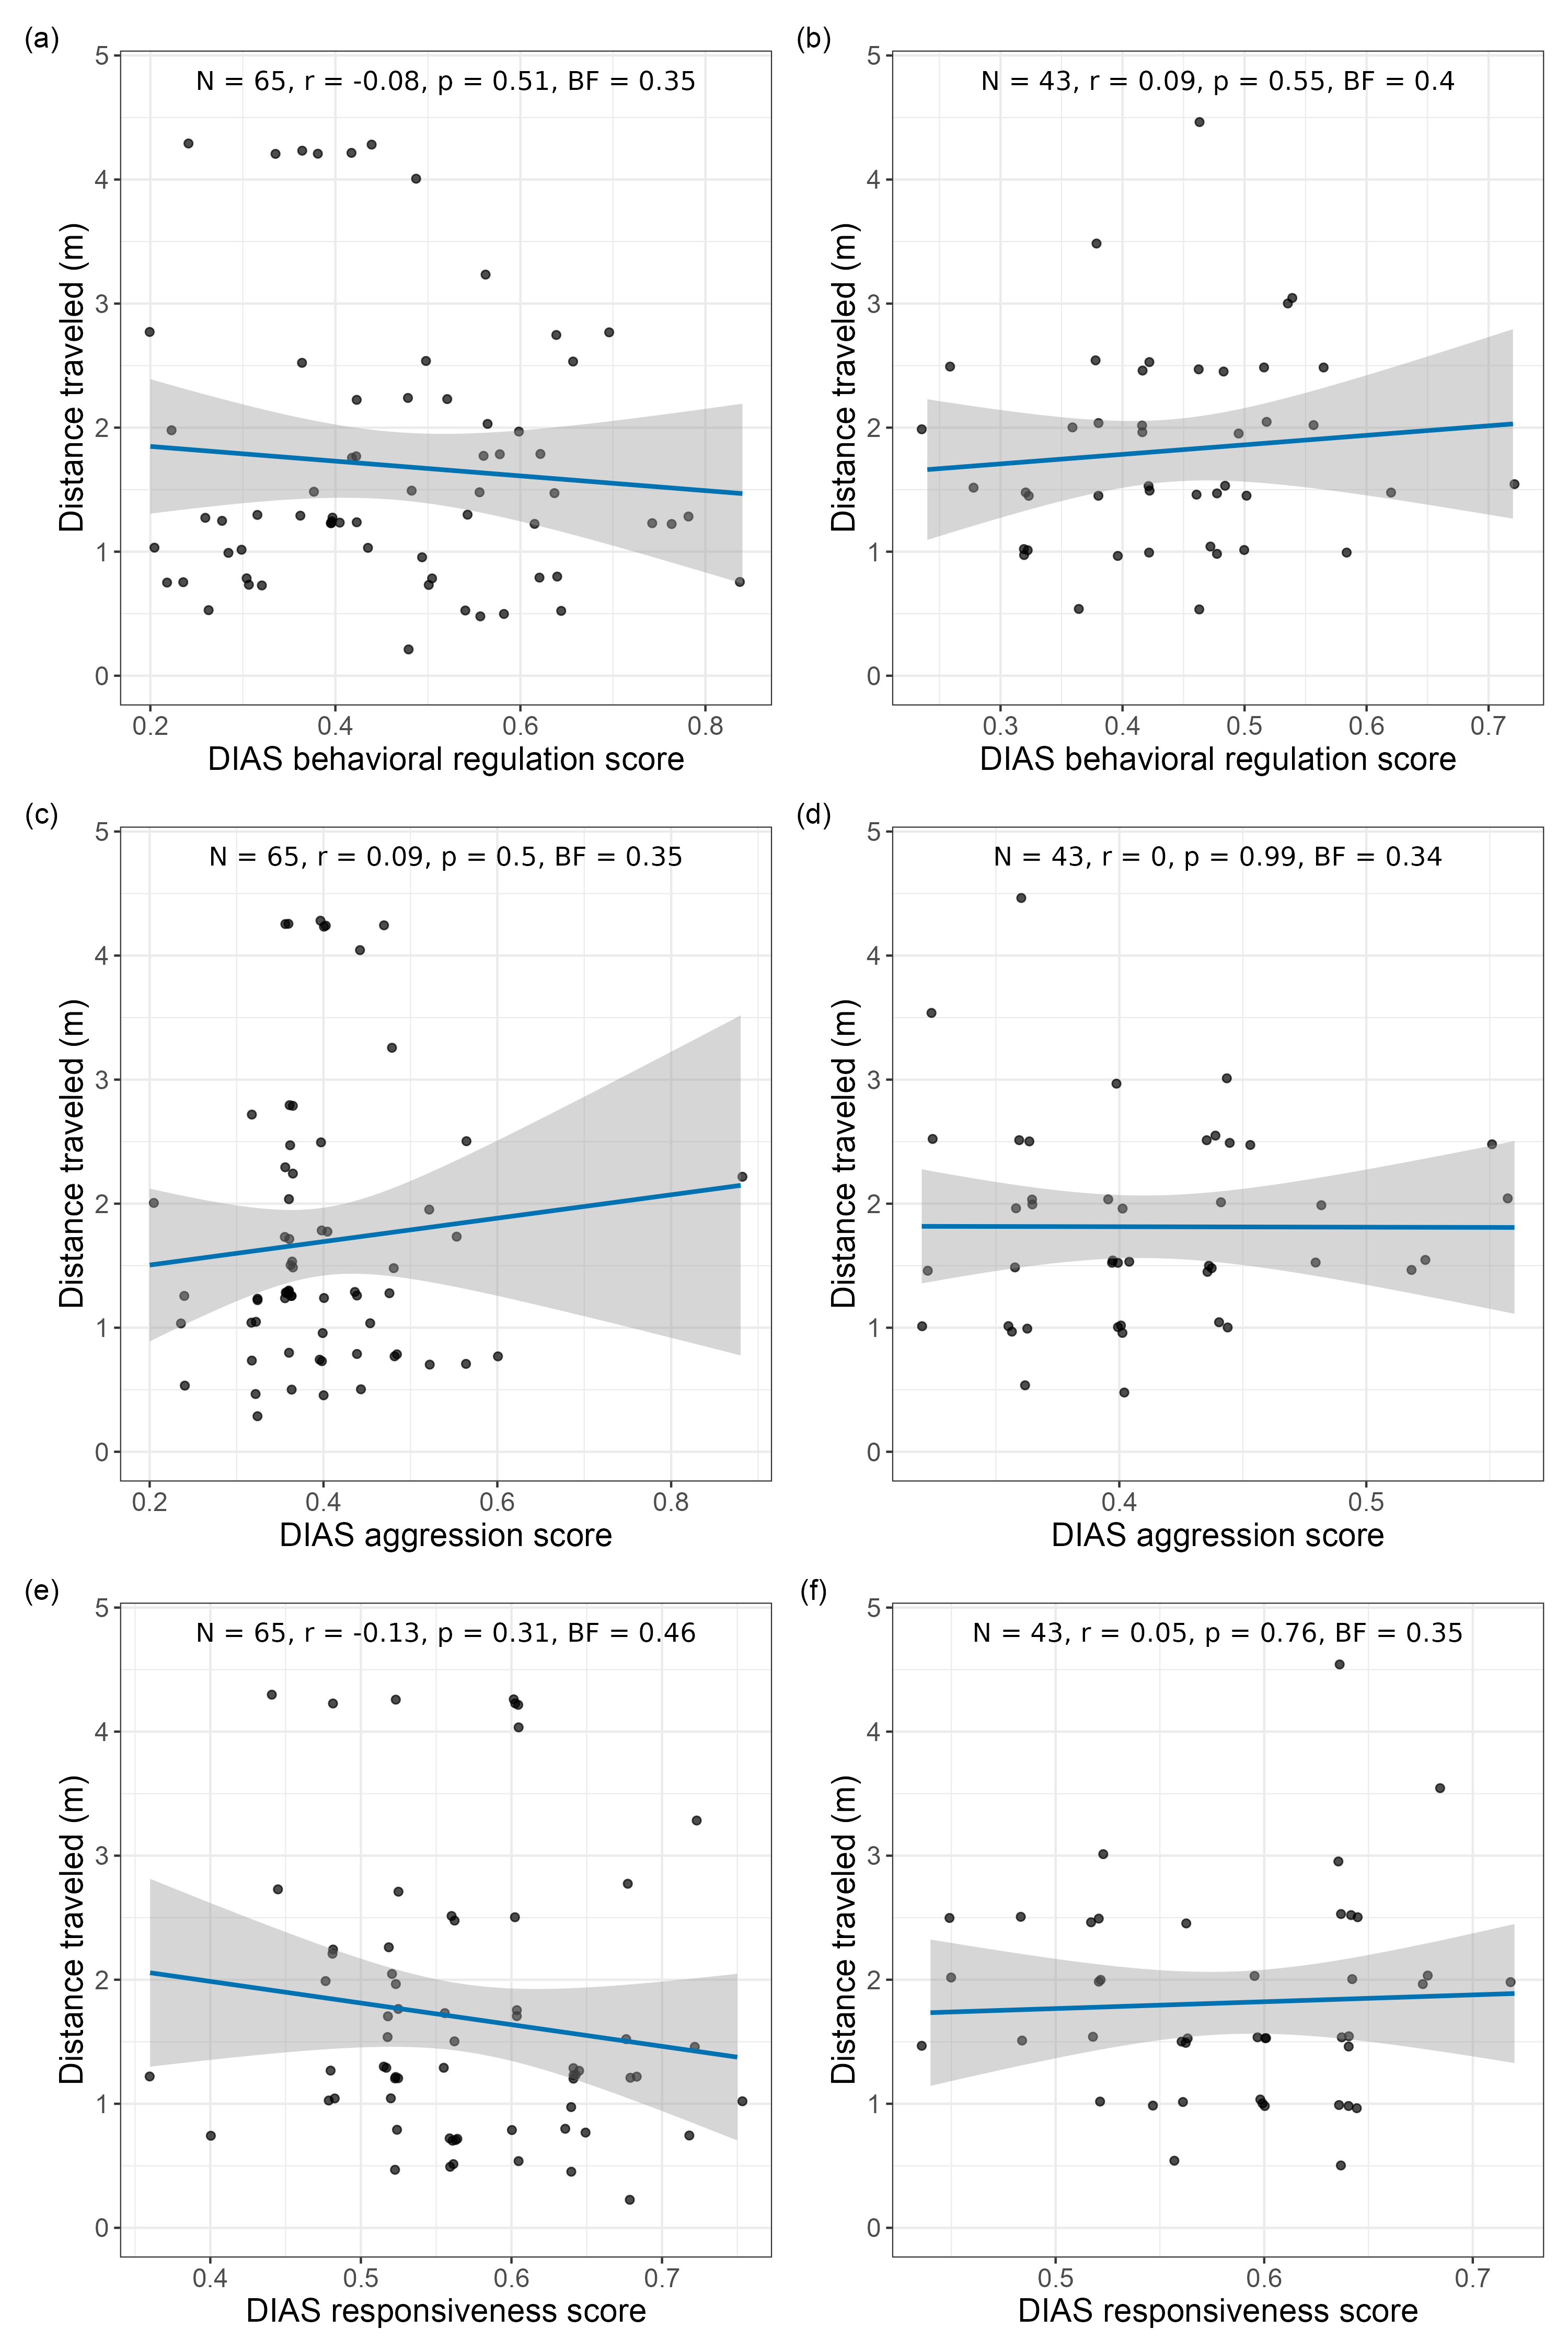
\includegraphics[width=0.75\linewidth]{figures/distance_dias_subscales} 

}

\caption{Relationship between distance traveled and DIAS subscales. We found no correlation between distance traveled and the behavioral regulation subscale in (a) Study 1 or (b) Study 2 or the aggression subscale in (c) Study 1 or (d) Study 2, or the responsiveness subscale in (e) Study 1 or (f) Study 2. Dots represent individual dog data points, lines represent best fitting linear regression models, and bands represent 95\% confidence intervals around the regression models. }\label{fig:dias-all}
\end{figure*}

\begin{figure*}

{\centering 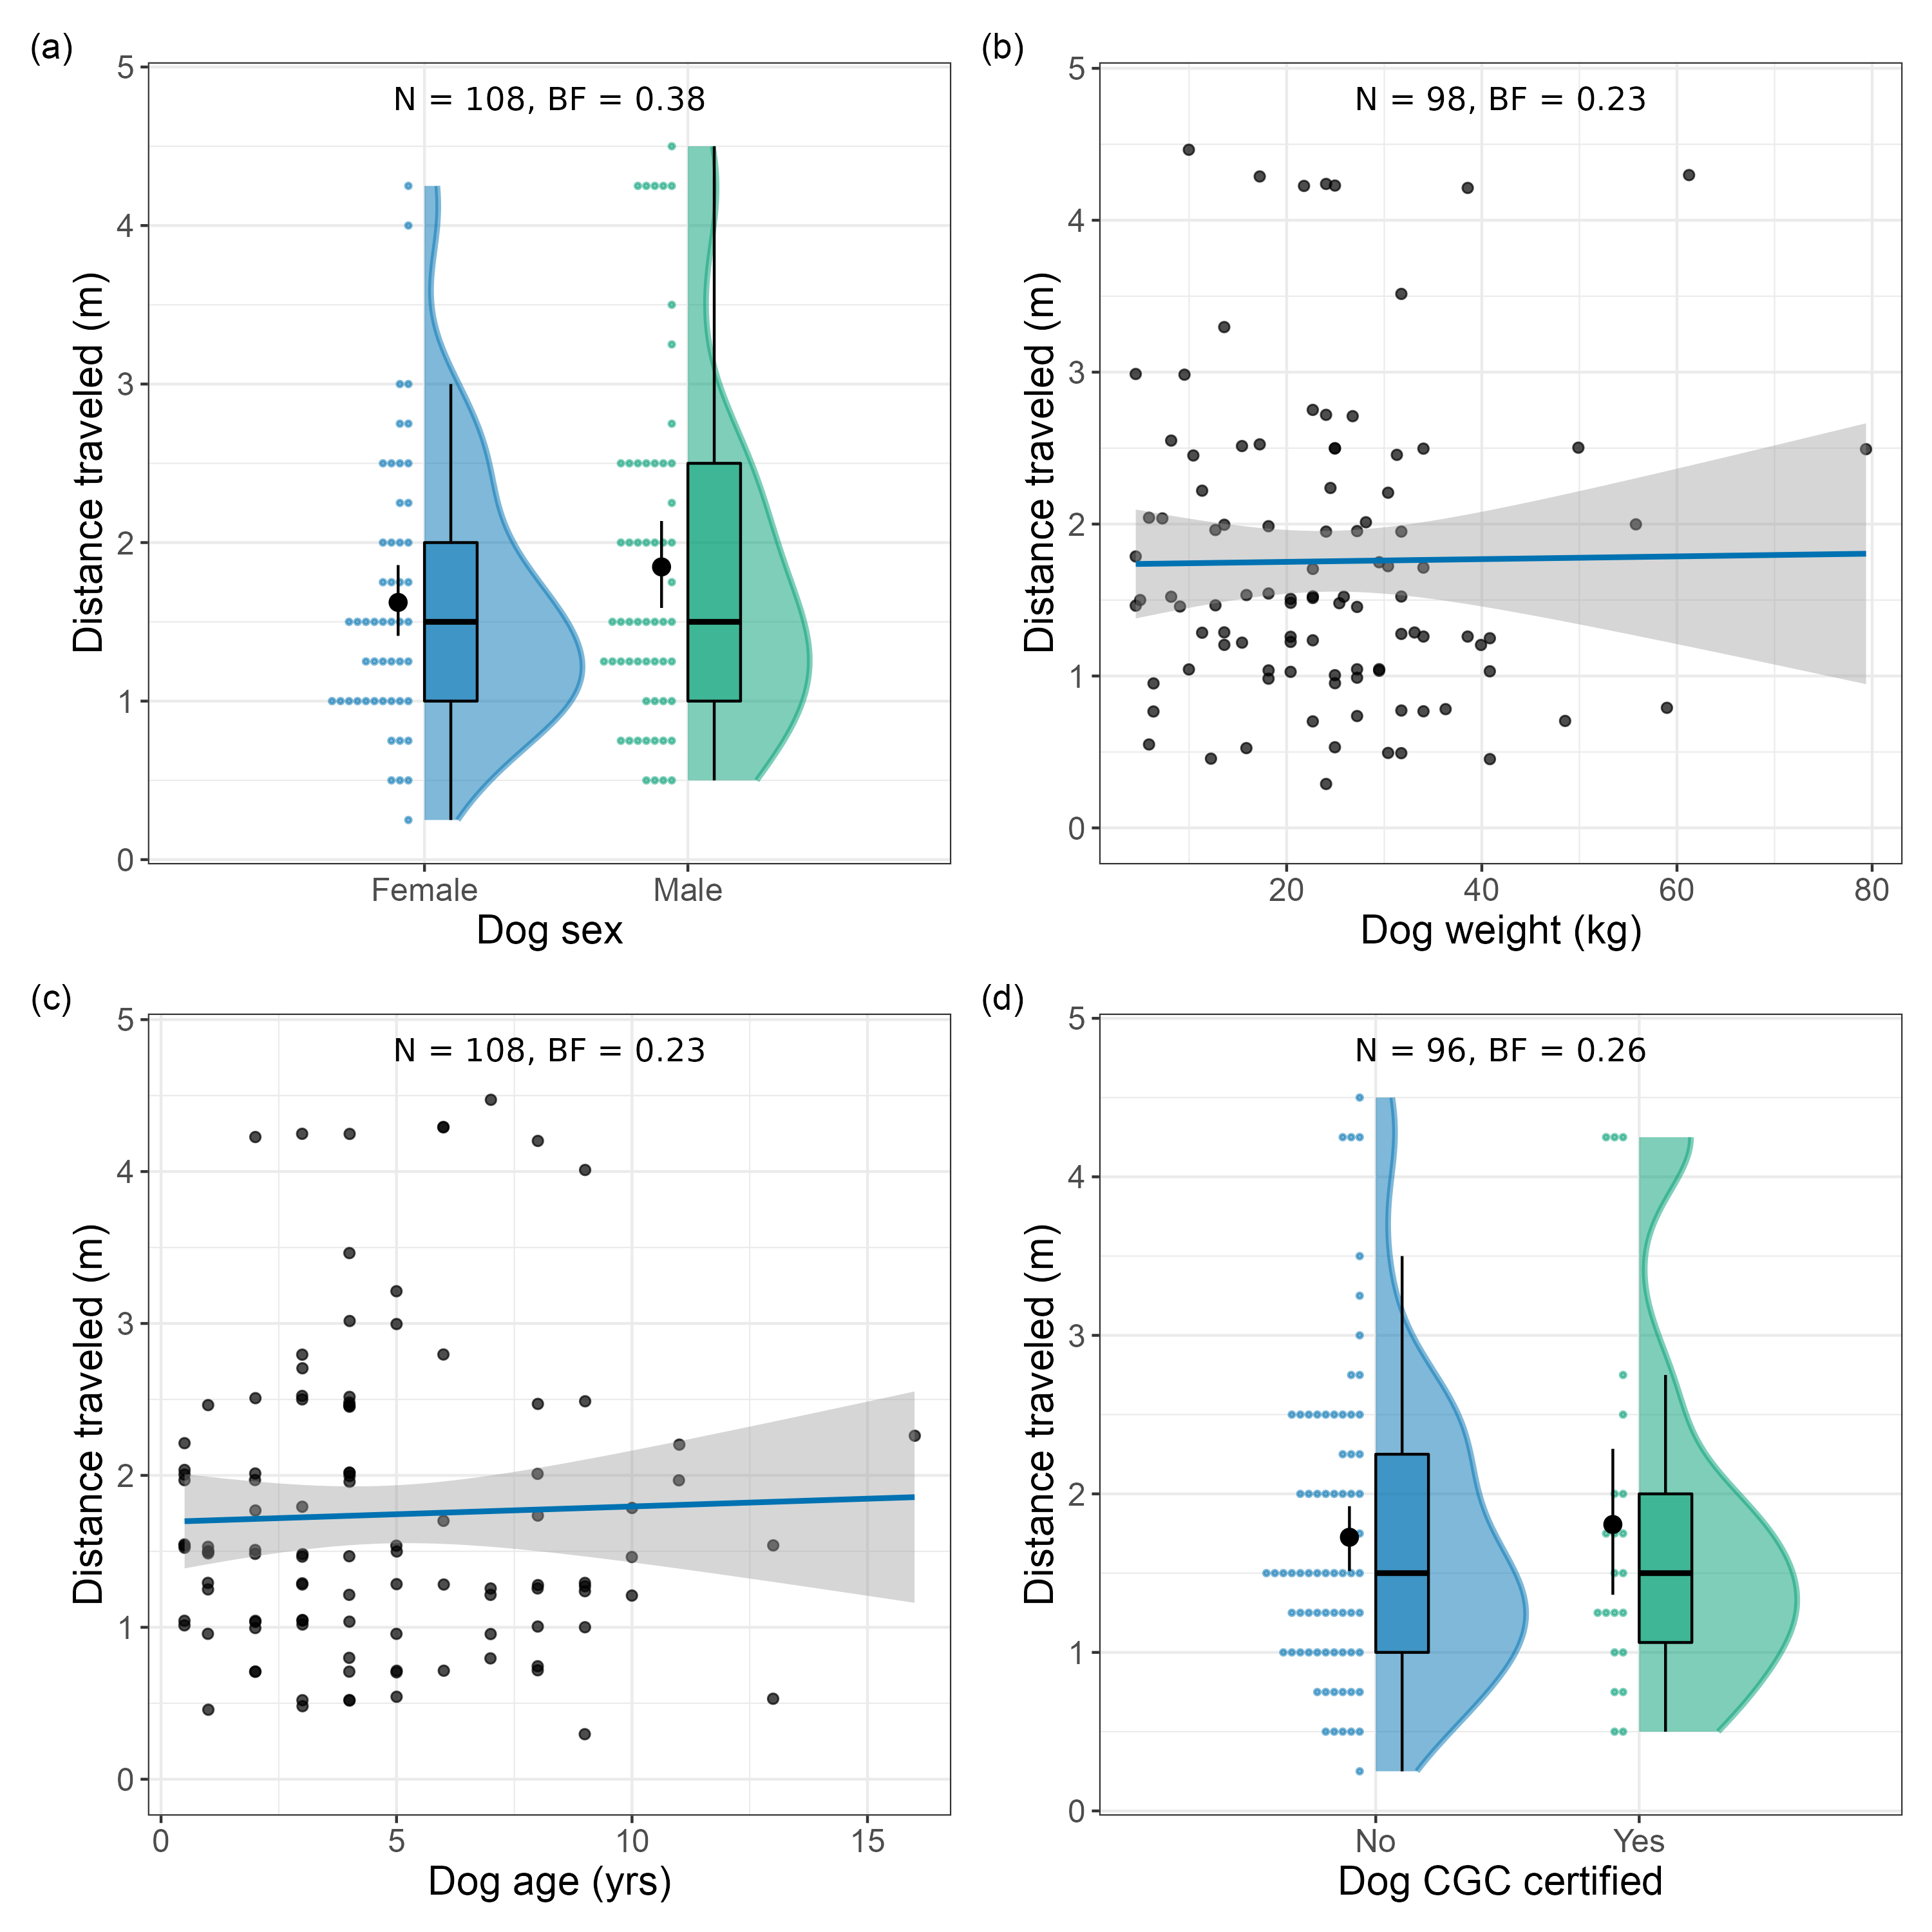
\includegraphics[width=0.95\linewidth]{figures/dog_characteristics} 

}

\caption{Relationship between distance traveled and dog characteristics. Distance traveled was not related to dog (a) sex, (b) weight, (c) age, or (d) AKC Canine Good Citizen status. For correlations, dots represent individual dog data points, lines represent best fitting linear regression models, and bands represent 95\% confidence intervals around the regression models. For group comparisons, dots represent individual dog data points, filled shapes represent density distributions, filled dots and error bars represent means and 95\% confidence intervals, boxes represent interquartile ranges, lines within boxes represent medians, and whiskers represent 1.5 times the interquartile range. }\label{fig:dog-char}
\end{figure*}

\begin{figure*}

{\centering 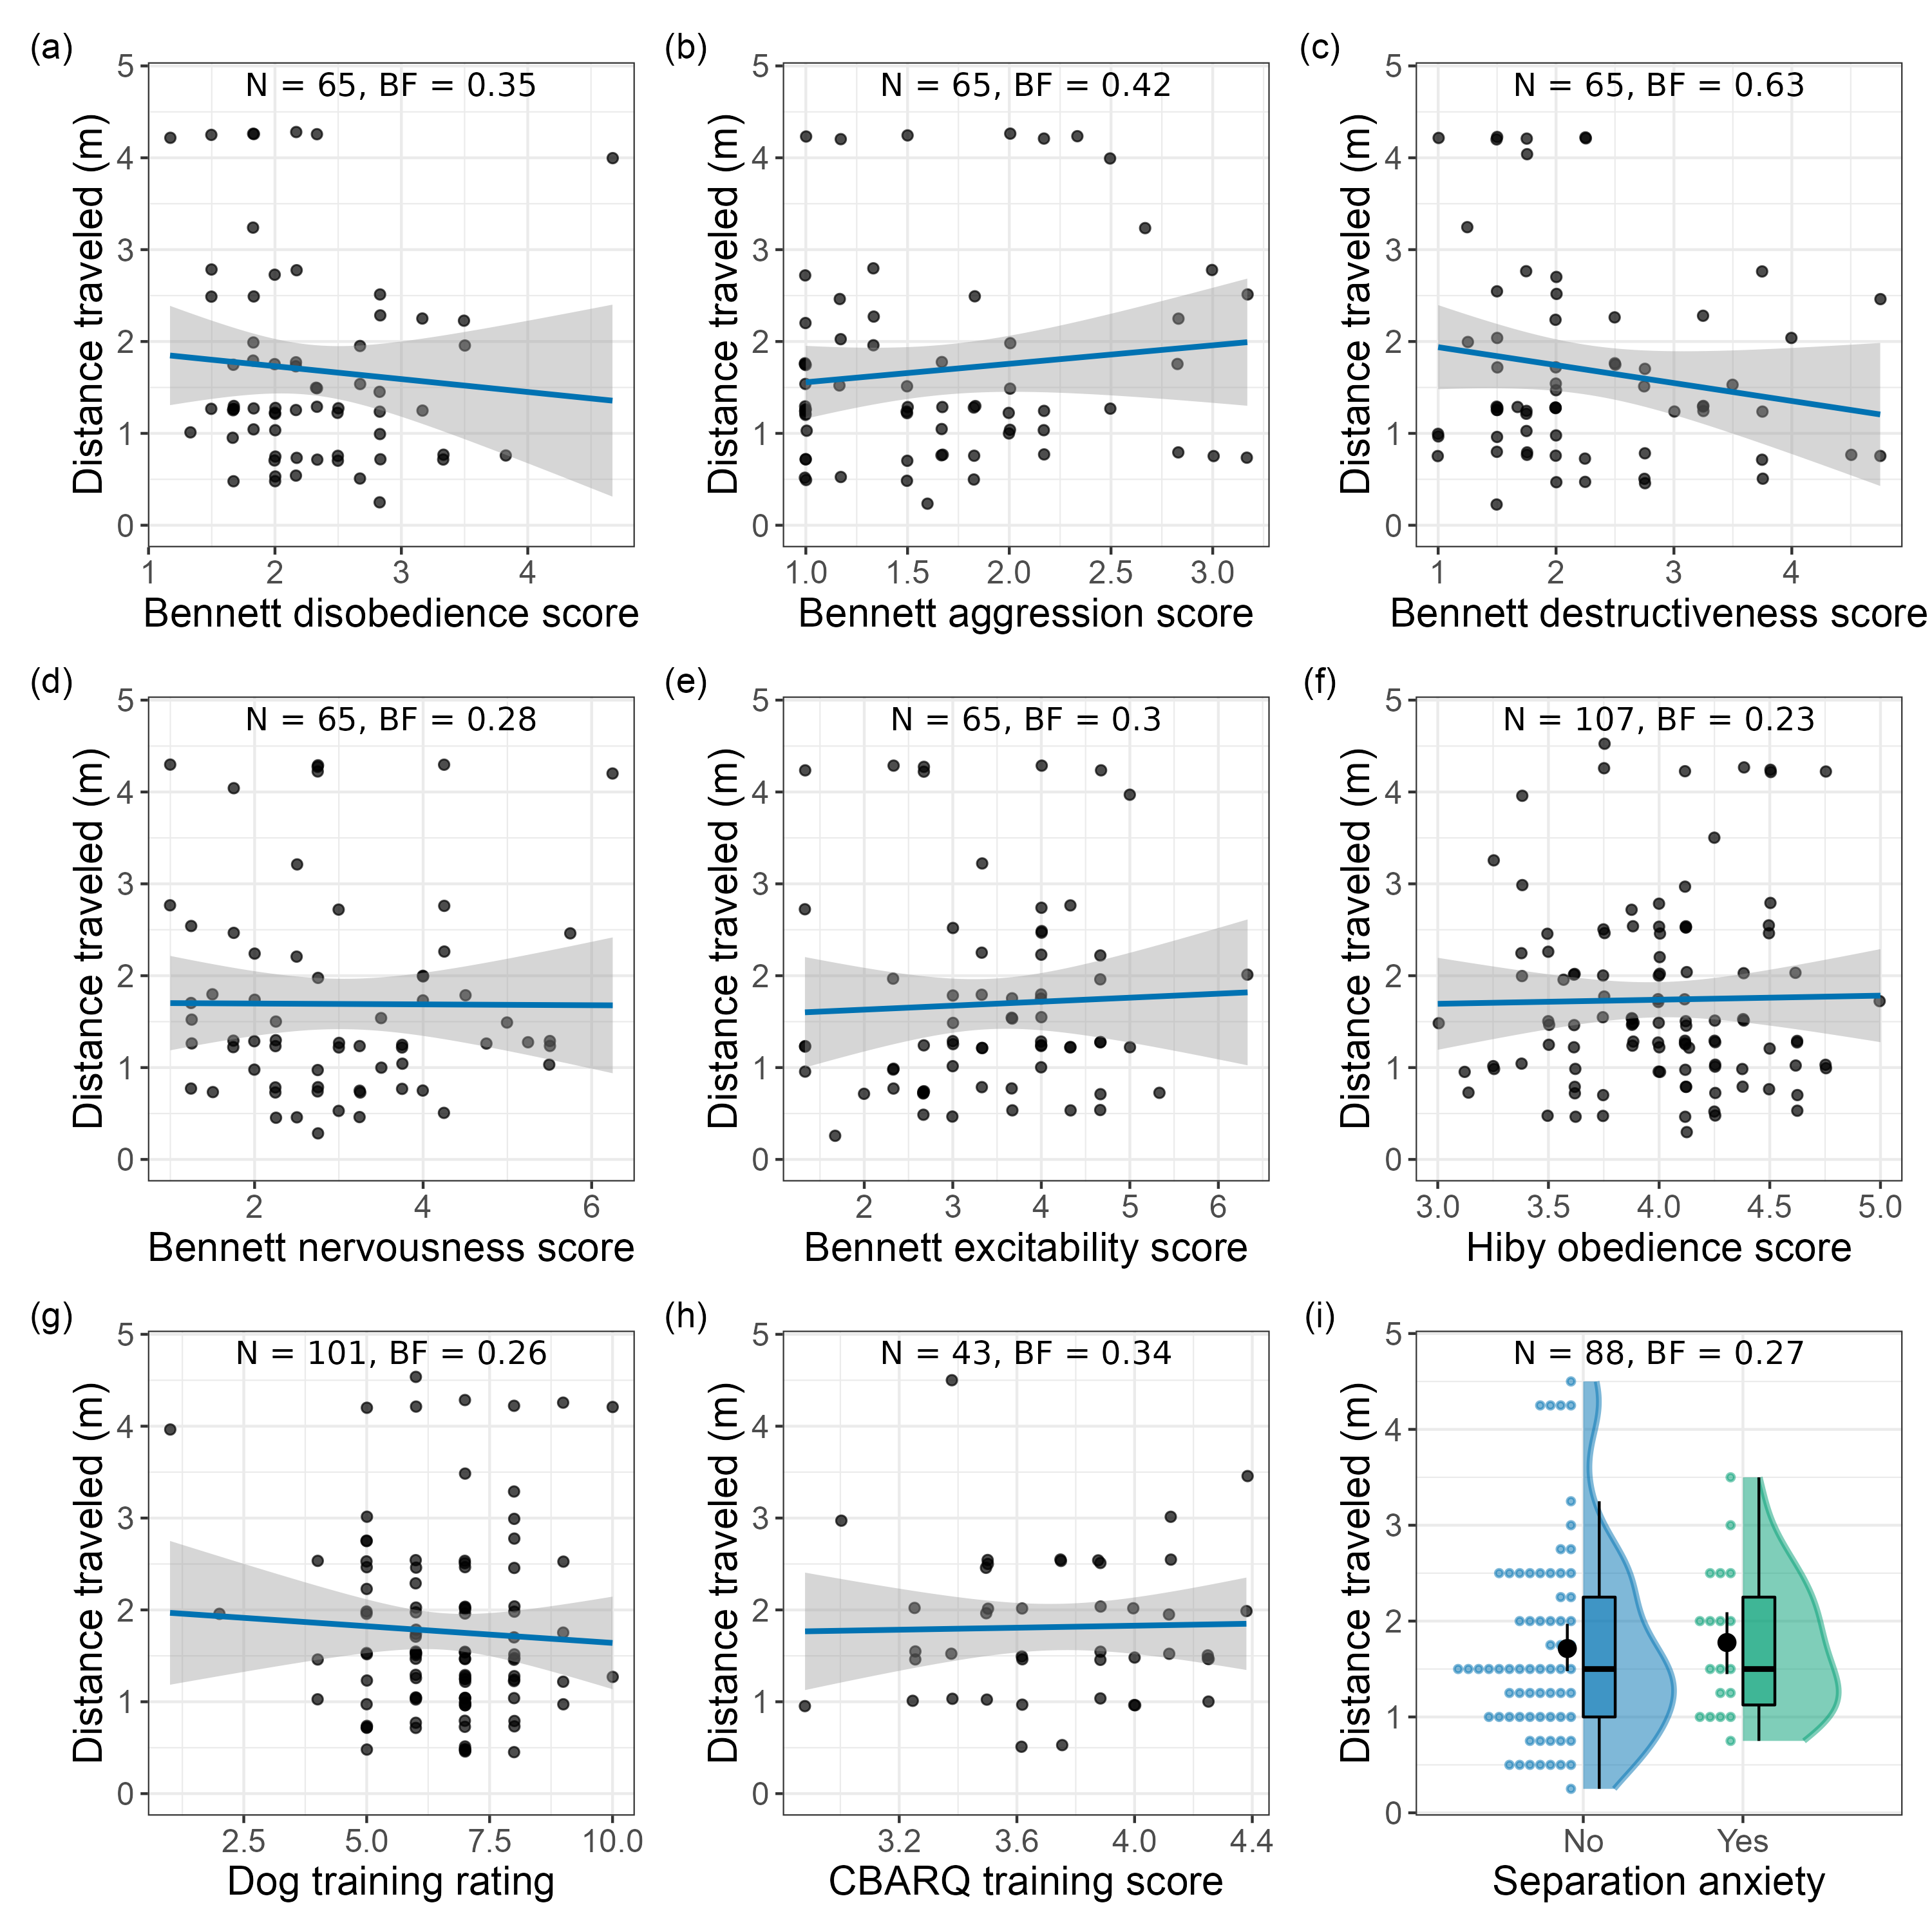
\includegraphics[width=0.95\linewidth]{figures/dog_behavior} 

}

\caption{Relationship between distance traveled and dog behavior. Distance traveled was not related to (a-e) scores on Bennett and Rolhf's (2007) behavior problems scales, (f) Hiby et al.'s (2004) obedience scale, (g-h) measures of training, or (i) ratings of separation anxiety. For correlations, dots represent individual dog data points, lines represent best fitting linear regression models, and bands represent 95\% confidence intervals around the regression models. For group comparisons, dots represent individual dog data points, filled shapes represent density distributions, filled dots and error bars represent means and 95\% confidence intervals, boxes represent interquartile ranges, lines within boxes represent medians, and whiskers represent 1.5 times the interquartile range. }\label{fig:dog-behavior}
\end{figure*}

\begin{figure*}

{\centering 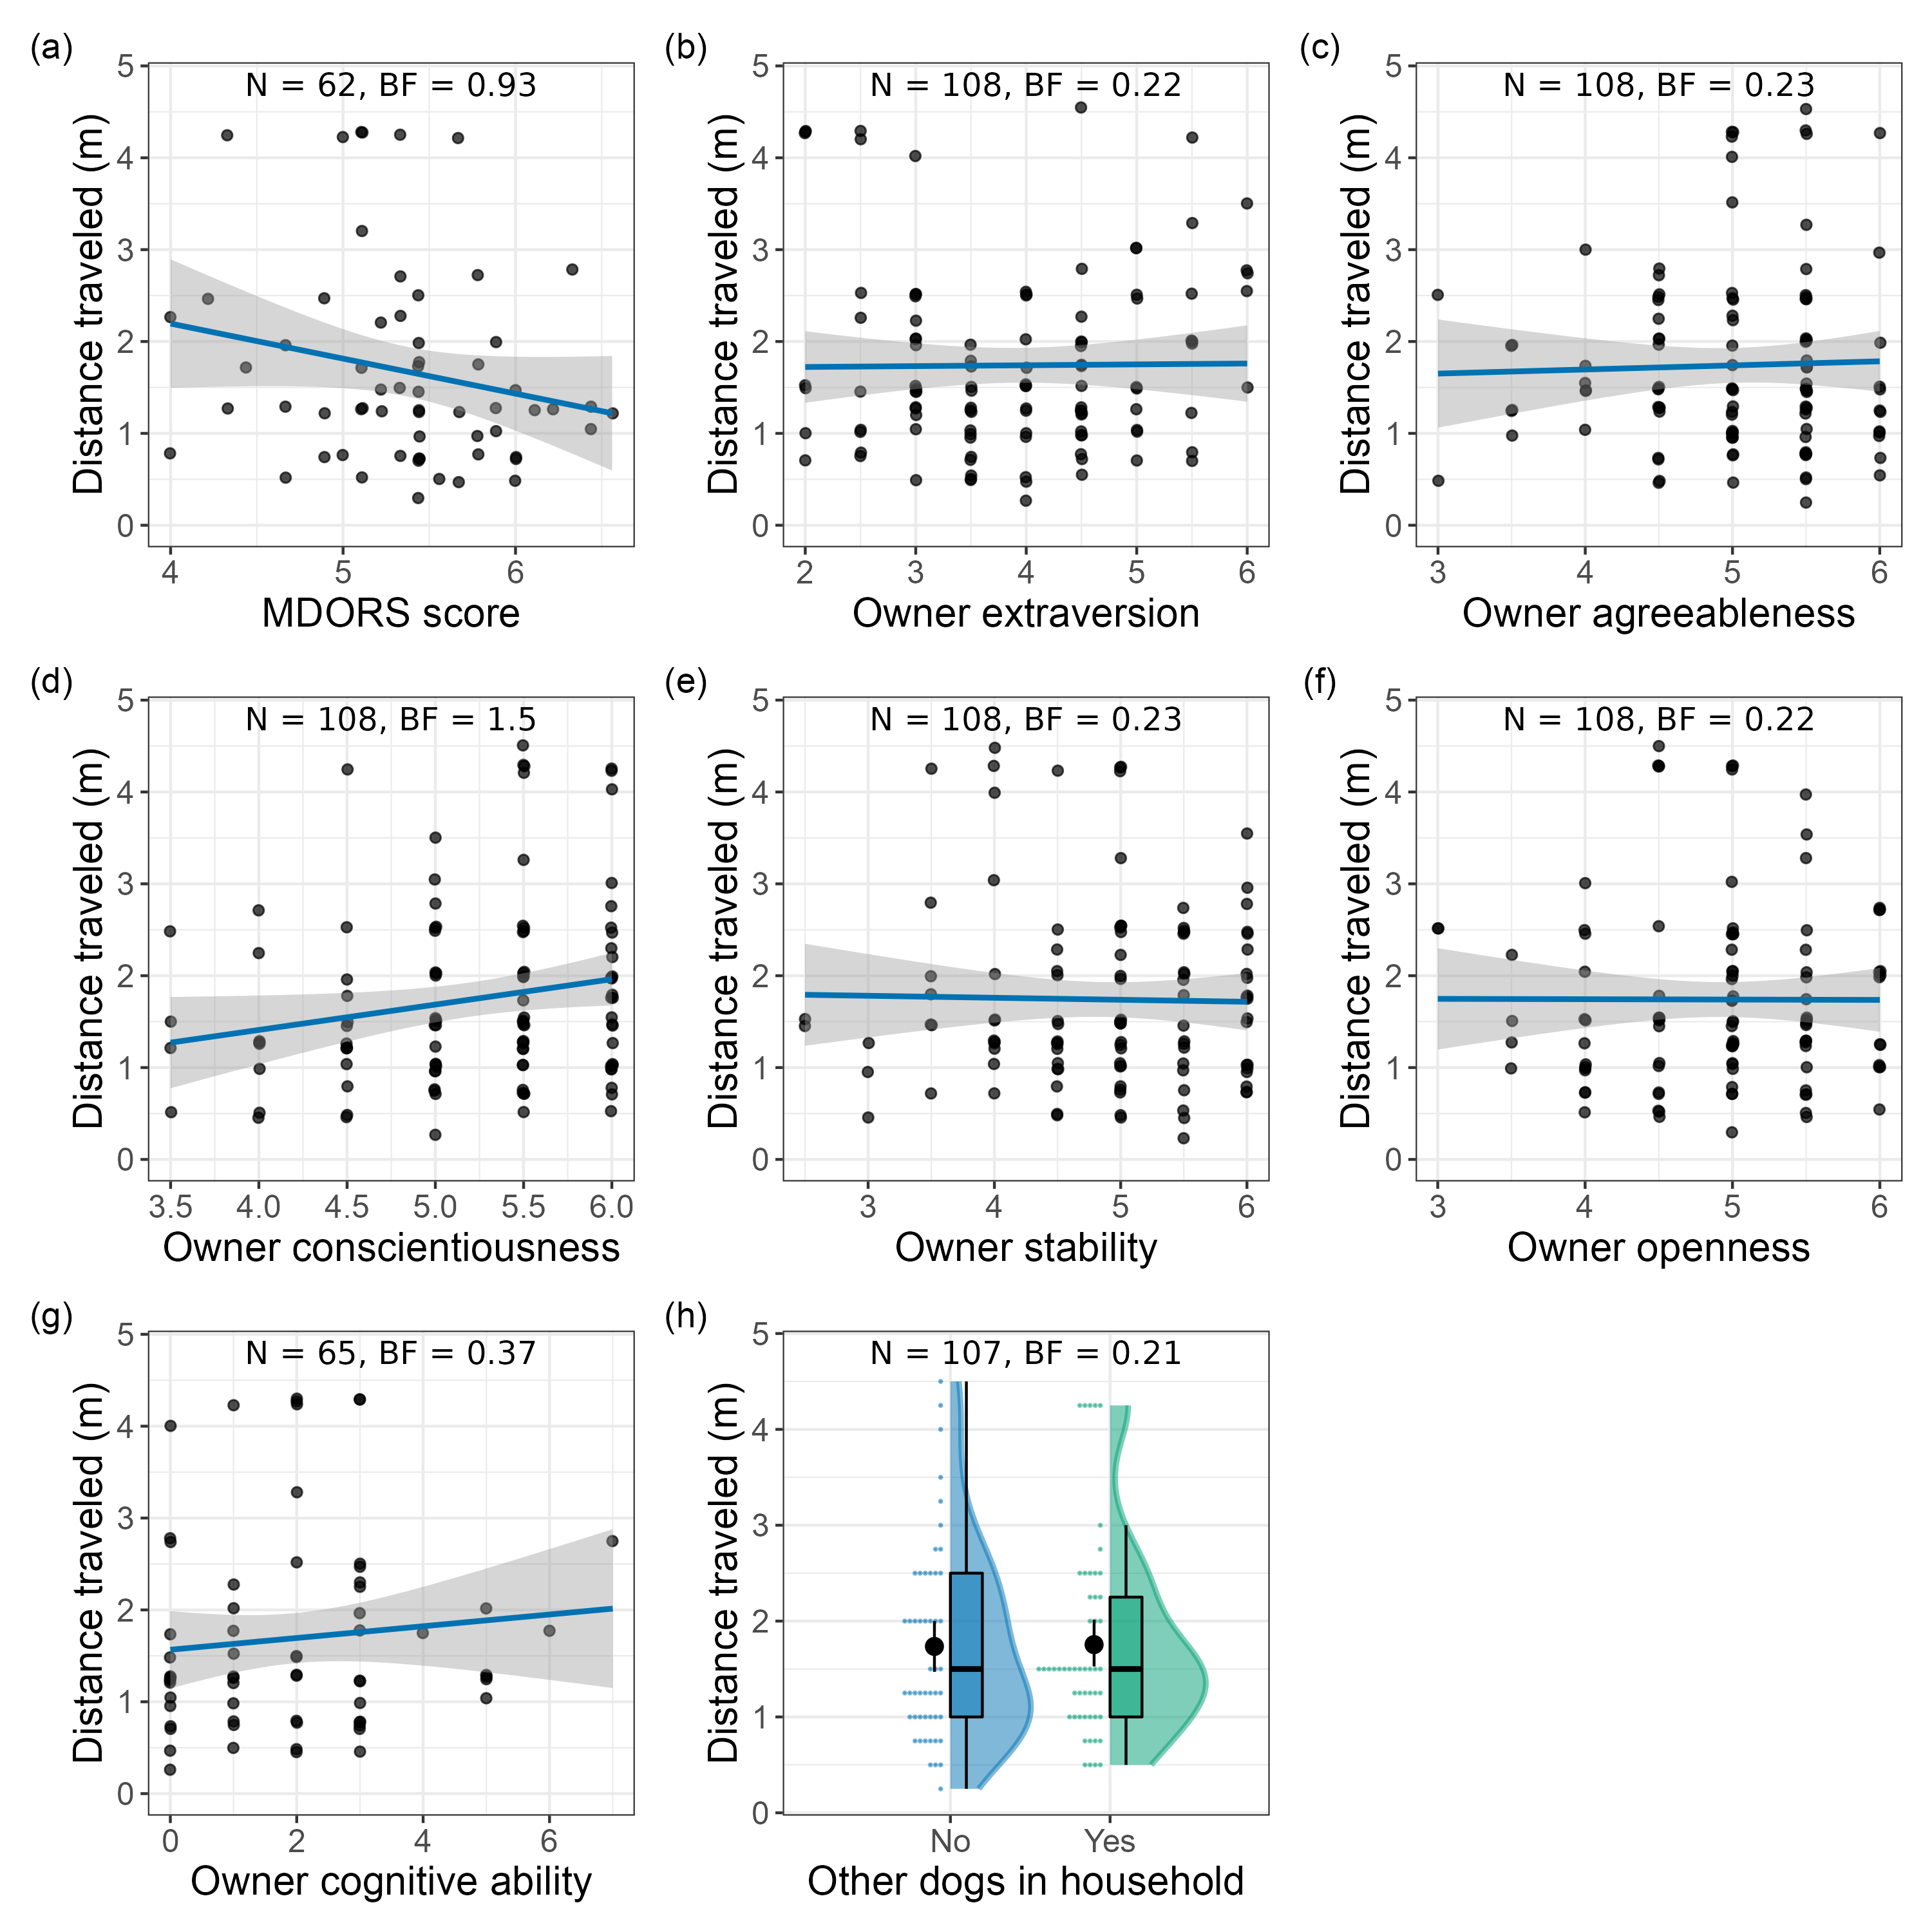
\includegraphics[width=0.95\linewidth]{figures/owner_characteristics} 

}

\caption{Relationship between distance travelled and owner characteristics. Distance traveled was not related to dog (a) Monash Dog Owner Relationship Score, (b-f) owner personality, (g) owner cognitive ability, or (h) whether owners had other dogs in the household. For correlations, dots represent individual dog data points, lines represent best fitting linear regression models, and bands represent 95\% confidence intervals around the regression models. For group comparisons, dots represent individual dog data points, filled shapes represent density distributions, filled dots and error bars represent means and 95\% confidence intervals, boxes represent interquartile ranges, lines within boxes represent medians, and whiskers represent 1.5 times the interquartile range. }\label{fig:owner-char}
\end{figure*}


\end{document}
